%% FEUP THESIS STYLE for LaTeX2e
%% how to use feupteses (English version)
%%
%% FEUP, JCL & JCF, 31 July 2012
%%
%% PLEASE send improvements to jlopes at fe.up.pt and to jcf at fe.up.pt
%%

%%========================================
%% Commands: pdflatex tese
%%           bibtex tese
%%           makeindex tese (only if creating an index) 
%%           pdflatex tese
%% Alternative:
%%          latexmk -pdf tese.tex
%%========================================

\documentclass[11pt,a4paper,twoside,openright]{report}

\usepackage{float}
\usepackage{afterpage}
\usepackage{listings}
\usepackage{import}
\usepackage{algorithm2e}
\usepackage{tabularx}
\usepackage[epsilon]{backnaur}
\usepackage{newfloat}

%% For iso-8859-1 (latin1), comment next line and uncomment the second line
\usepackage[utf8]{inputenc}
%\usepackage[latin1]{inputenc}
\usepackage[portuguese,english]{babel}

%% English version

%% MIEIC options
%\usepackage[mieic]{feupteses}
\usepackage[mieic,juri]{feupteses}
%\usepackage[mieic,final]{feupteses}
%\usepackage[mieic,final,onpaper]{feupteses}

%% Additional options for feupteses.sty: 
%% - onpaper: links are not shown (for paper versions)
%% - backrefs: include back references from bibliography to citation place

%% Uncomment the next lines if side by side graphics used
%\usepackage[lofdepth,lotdepth]{subfig}
%\usepackage{graphicx}
%\usepackage{float}

%% Include color package
\usepackage{color}
\definecolor{cloudwhite}{cmyk}{0,0,0,0.025}

% declare the floating environment {Grammar}
% this will also define \listofGrammars:
\DeclareFloatingEnvironment[
  % the file extension for the file used to create the list:
  fileext   = logr,% don't use log here!
  % the heading for the list:
  listname  = {List of Grammars},
  % the name used in captions:
  name      = Grammar,
  % the default floating parameters if the environment is used
  % without optional argument:
  placement = htp
]{Grammar}

%% Include source-code listings package
\usepackage{listings}
\lstset{ %
 language=C,                        % choose the language of the code
 basicstyle=\footnotesize\ttfamily,
 keywordstyle=\bfseries,
 numbers=left,                      % where to put the line-numbers
 numberstyle=\scriptsize\texttt,    % the size of the fonts that are used for the line-numbers
 stepnumber=1,                      % the step between two line-numbers. If it's 1 each line will be numbered
 numbersep=8pt,                     % how far the line-numbers are from the code
 frame=tb,
 float=htb,
 aboveskip=8mm,
 belowskip=4mm,
 backgroundcolor=\color{cloudwhite},
 showspaces=false,                  % show spaces adding particular underscores
 showstringspaces=false,            % underline spaces within strings
 showtabs=false,                    % show tabs within strings adding particular underscores
 tabsize=2,	                    % sets default tabsize to 2 spaces
 captionpos=b,                      % sets the caption-position to bottom
 breaklines=true,                   % sets automatic line breaking
 breakatwhitespace=false,           % sets if automatic breaks should only happen at whitespace
 escapeinside={\%*}{*)},            % if you want to add a comment within your code
 morekeywords={*,var,template,new}  % if you want to add more keywords to the set
}

%% Uncomment to create an index (at the end of the document)
%\makeindex

%% Path to the figures directory
%% TIP: use folder ``figures'' to keep all your figures
\graphicspath{{figures/}}

%%----------------------------------------
%% TIP: if you want to define more macros, use an external file to keep them
%some macro definitions

% format
\newcommand{\class}[1]{{\normalfont\slshape #1\/}}

% entities
\newcommand{\Feup}{Faculdade de Engenharia da Universidade do Porto}

\newcommand{\svg}{\class{SVG}}
\newcommand{\scada}{\class{SCADA}}
\newcommand{\scadadms}{\class{SCADA/DMS}}

%%----------------------------------------

%%========================================
%% Start of document
%%========================================
\begin{document}

%%----------------------------------------
%% Information about the work
%%----------------------------------------
\title{Reverse Engineering of Interaction Patterns}
\author{Clara Sacramento}

%% Uncomment next line for date of submission
%\thesisdate{July 31, 2008}

%%Uncomment next line for copyright text if used
%\copyrightnotice{Name of the Author, 2008}

\supervisor{Supervisor}{Ana Paiva (PhD)}

%% Uncomment next line if necessary
%\supervisor{Second Supervisor}{Name of the Supervisor}

%% Uncomment committee stuff in the final version if used
%\committeetext{Approved in oral examination by the committee:}
%\committeemember{Chair}{Doctor Name of the President}
%\committeemember{External Examiner}{Doctor Name of the Examiner}
%\committeemember{Supervisor}{Doctor Name of the Supervisor}
%\signature

%% Specify cover logo (in folder ``figures'')
\logo{uporto-feup.pdf}

%% Uncomment next line for additional text  below the author's name (front page)
%\additionalfronttext{Preparação da Dissertação}

%%----------------------------------------
%% Preliminary materials
%%----------------------------------------

% remove unnecssary \include{} commands
\begin{Prolog}
  \chapter*{}

This work is financed by the ERDF - European Regional Development Fund through the COMPETE Programme (operational programme for competitiveness) and by National Funds through the FCT - Fundação para a Ciência e a Tecnologia (Portuguese Foundation for Science and Technology) within project FCOMP-01-0124-FEDER-020554.

\begin{figure}[!b]
  \begin{center}
    \leavevmode
    
\includegraphics[width=\textwidth]{acks}
    \label{fig:arch}
  \end{center}
\end{figure}  % the FCT
  \chapter*{Abstract}
A great deal of effort in model-based testing is related to the creation of the model. In addition, the model itself, while a powerful tool of abstraction, can have conceptual errors, introduced by the tester. These problems can be reduced by generating those models automatically. This dissertation presents a dynamic reverse engineering approach that aims to extract part of the model of an existing Web application through the identification of User Interface (UI) patterns. This reverse engineering approach explores automatically any Web application, records information related to the interaction, analyzes the gathered information, tokenizes it, and infers the existing UI patterns via syntactical analyzing. After complemented with additional information and validated, the model extracted is the input for the Pattern-Based Graphical User Interface Testing (PBGT) approach for testing existing web application under analysis.

First the theme developed during the course of the dissertation is introduced, starting by defining the context and issue at hand and describing the goals of this dissertation. Afterwards we present a literary review on reverse engineering approaches, approaches that infer patterns from Web applications, and data mining algorithms and tools relevant to the problem. We explain the approach in detail, present a case study, and lastly, we present the conclusions taken from the work.

\chapter*{Resumo}
\begin{otherlanguage}{portuguese}
Grande parte do esforço despendido em testes baseados num modelo está relacionado com a criação do modelo. Além disso, o modelo, mesmo sendo uma ferramenta poderosa de abstração, pode ter erros conceptuais introduzidos pelo testador. Esses problemas podem ser reduzidos ao gerar esses modelos automaticamente. Esta dissertação apresenta uma abordagem de engenharia reversa dinâmica que pretende extrair parte do modelo de uma aplicação Web a testar, diretamente da sua interface gráfica, através da identificação de padrões de interface de utilizador (\textit{UI Patterns}). Esta abordagem de engenharia reversa explora automaticamente qualquer aplicação Web, guarda informação relacionada com a interação, analisa a informação guardada, analisa-a lexicalmente, e infere padrões através de análise sintáctica. Após ser complementado com informação adicional e validado, o modelo resultante serve de entrada para a abordagem de Teste de GUIs baseado em Padrões (PBGT), para testar a aplicação Web sobre análise.

Primeiro o tema desenvolvido no decorrer da dissertação é introduzido, começando por definir o seu contexto, motivação e objectivos. Depois é apresentada uma revisão bibliográfica de abordagens que usam engenharia reversa e abordagens que inferem padrões de aplicações Web.  A abordagem desenvolvida é apresentada em detalhe, é apresentado um caso de estudo, e finalmente são apresentadas as conclusões do trabalho realizado.
\end{otherlanguage} % the abstract
  \chapter*{Acknowledgements}

First of all, I would like to thank my supervisor, Ana Paiva, from the Faculty of Engineering of University of Porto, for her guidance, insight, encouragement and support during the whole masters. Our weekly moments of discussion were indispensable for the success of this work, and specially for keeping me in the right track and focused on what was important (and not what it would be cool to do).

I would also like to thank all my teachers, from the first grade to my last year in college, as without them I wouldn't have had the necessary skills to accomplish this.

My friends’ friendship has been very important to me and so I thank them for being there for me every step of the way. I would like to specially thank the members of NIAEFEUP, with a very special mention for Pedro, for all the talking, all the comfort and teasing, all the help, and the kind words in the darkest moments. Thank you for all the great moments we have spent together, and for all that we have accomplished together.

A special thank to my parents, Maria and Adelino, without whom I would not be the person I am today and would have not achieved all the great things I have in my life. Thank you for all of your love, your concern and specially your loving support. Thank you for being there for me around the clock.

And finally, a special thank to my boyfriend, Diogo. Thank you for your insight in some of my assignments. Thank you for all of your love, your friendship, the comfort you provided me, your understanding, your patience and for every time you have teased me
along the years.

%\vspace{10mm}
%\flushleft{Clara Raquel da Costa e Silva Sacramento}  % the acknowledgments
  \cleardoublepage
\thispagestyle{plain}

\vspace*{8cm}

\begin{flushright}
   \textsl{``You should be glad that bridge fell down. \\
           I was planning to build thirteen more to that same design''} \\
\vspace*{1.5cm}
           Isambard Kingdom Brunel
\end{flushright}
       % initial quotation if desired
  \cleardoublepage
  \pdfbookmark[0]{Table of Contents}{contents}
  \tableofcontents
  \cleardoublepage
  \pdfbookmark[0]{List of Figures}{figures}
  \listoffigures
  \cleardoublepage
  \pdfbookmark[0]{List of Tables}{tables}
  \listoftables
  \cleardoublepage
  \pdfbookmark[0]{List of Algorithms}{algorithms}
  \listofalgorithms
  \chapter*{Abbreviations}
\chaptermark{ABBREVIATIONS}

\begin{flushleft}
\begin{tabular}{l p{0.8\linewidth}}
FEUP	& \Feup{} \textit{(Faculdade de Engenharia da Universidade do Porto)}\\
RIA	& Rich Internet Applications \\
API	& Application Programming Interface \\
%AST	& Abstract Syntax Tree \\
DSL	& Domain Specific Language \\
AUA	& Application Under Analysis \\
CIO	& Concrete Interaction Objects \\
EFG	& Event Flow Graph \\
%FSM	& Finite State Machine \\
GUI	& Graphical User Interface \\
%MBT	& Model-Based Testing \\
SUT	& System Under Testing \\
TDD	& Test-Driven Development \\
UI	& User Interface \\
HTML	& HyperText Markup Language \\
UML	& Unified Modeling Language \\
%AUIDL	& Abstract UI Description Language \\
%HCI	& Human Computer Interaction \\
REGUI	& Reverse Engineering of Graphical User Interface \\
%V\&V	& Verification and Validation \\
XML	& eXtensible Markup Language \\
\end{tabular}
\end{flushleft}

  % the list of abbreviations used
\end{Prolog}

%%----------------------------------------
%% Body
%%----------------------------------------
\StartBody

%% TIP: use a separate file for each chapter
\chapter{Introduction} \label{chap:intro}

\section*{}

\section{Context} \label{sec:context}

Web applications are getting more and more important. Due to their stability and security against losing data, there is a growing trend to move applications towards the Web, with the most notorious examples being Google's mail and office software applications. Web applications can now handle tasks that before could only be performed by desktop applications \cite{garrett2005ajax}, like editing images or creating spreadsheet documents.

Despite the relevance that Web applications have in the community, they still suffer from a lack of standards and conventions \cite{constantine2002usage}, unlike desktop and mobile applications. This means that the same task can be implemented in many different ways, which makes automated testing difficult to accomplish and inhibits reuse of testing code. For instance, authentication (\textit{login}) failure usually triggers the appearance of an error message, but some implementations simply erase the inserted data, with no error message visible.

GUIs \textit{(Graphical User Interfaces)} of all kinds are populated with recurring behaviors that vary slightly; examples being authentication via \textit{login/password} pair and content search. These behaviors (patterns) are called User Interface (UI) patterns \cite{van2001patterns} and are recurring solutions to common design problems. Due to their widespread use, UI patterns allow users a sense of familiarity and comfort when using applications.

However, while UI patterns are familiar to users, their implementation may vary significantly. Despite this, it is possible to define generic and reusable test strategies (User Interface Test Patterns - UITP) to test those patterns. This requires a configuration process, in order to adapt the tests to different applications \cite{dalal1999model}.

Testing is an increasingly important part of any development process as it is essential to improve the trust in the quality of software. Thus, there is an ever increasing need to develop new techniques in this field. This necessity is increased by the constant improvement of development techniques.

When it comes to GUI testing, there are some applicable testing techniques \cite{memon2002gui}: \textbf{capture replay}, which requires a functional GUI; \textbf{unit testing}, which requires the manual implementation of the tests and may involve too much work in order to test all of the functionalities; \textbf{random input testing}, which is good at finding situations where the system crashes, but is not as good at finding other kinds of errors; and \textbf{model-based testing}, which enables automatic test case generation and execution, even though it requires a formal model in order to generate the test cases.

\section{Motivation and Objectives} \label{sec:goals}

As mentioned before, the focus of this dissertation is a component of a research project named PBGT (\textit{Pattern-based GUI Testing}) \cite{moreira2013pattern}. The main goal of of this project is to improve current model-based GUI testing methods and tools, contributing to conceive an effectively applicable testing approach in industry and to contribute to the construction of higher quality GUIs and software systems. One of the problems to overcome when implementing a model-based GUI testing approach is the time required to construct the model and the test case explosion problem. Choosing the right abstraction level of the model, extracting part of that model by a reverse engineering process and focusing the test cases to cover common recurrent behavior seems to be a way to solve these problems.

The proposal aims to continue the work done on PARADIGM-RE, a component of the PBGT process responsible for extracting part of the Web application model from the Web application itself via reverse engineering, by developing a completely new tool to extract a partial model of a Web application via reverse engineering.

The previous tool \cite{nabuco2013inferring,nabuco2014inferring} is a dynamic reverse engineering approach that extracts User Interface (UI) Patterns from existent Web applications. Its functioning can be summed up like this: 

\begin{itemize}
\item First, the user interacts with the Web application, navigating it to the best of his ability while the tool records information related to the interaction (user actions and parameters, and for each page visited, its HTML source and URL);
\item Second, the collected information is analyzed in order to calculate several metrics (e.g., the differences between subsequent HTML pages);
\item Lastly, the existent UI Patterns are inferred from the overall information calculated based on a set of heuristic rules.
\end{itemize}

This approach was evaluated on several widely used Web applications and the results were deemed satisfactory, since the tool identified most of the occurring patterns and their location on the page. However, there are some patterns the tool doesn't identify, such as the Menu pattern, and the heuristics are considered to be still in an incipient state. The tool's major weakness is that it requires a user to interact with a Web application, a process that can quickly become morose and time-consuming.

As stated before, this dissertation aims to develop a new tool for extracting a partial model from a Web aplication meant to be tested. The major goals for this dissertation were to improve the existing reverse engineering and pattern inferring process, remove the need for user interaction, and automate the model construction; or in other words, independently/automatically explore a Web application, infer the existing UI patterns in its pages, and finally produce a model with the UI Test Patterns that define the strategies to test the UI Patterns present in the web application. This is meant to speed up model construction, and mitigate the number of errors introduced into the model.

\section{Structure of the Report} \label{sec:outline}

This document is structured into four main chapters. In this first section, Chapter \ref{chap:intro}, we start by introducing the theme to be developed during the course of the dissertation, define the context, motivations, goals of this dissertation and the issue at hand. Chapter \ref{chap:sota} introduces essential concepts to understand the problems with which this document deals, and presents the state of the art on reverse engineering. Chapter \ref{chap:approach} presents the developed tool, RE-TOOL, focusing on its architecture and functionalities and on some of the challenges which needed to be tackled during the development. Chapter \ref{chap:validation} presents a case study. Finally, Chapter \ref{chap:conclusion} presents some conclusions about this research work, along with the limitations of the implementation. 
\chapter{State-of-the-Art} \label{chap:sota}

\section*{}

\section{Introduction}
In order to find the best approach to this problem, some research on already existing methodologies and concepts was needed. First an overview for the general categories researched is given, followed by the actual state of the art found, divided by relevant subcategories. 

\section{Reverse Engineering}\label{sec:reverseengineering}

Reverse engineering is “the process of analyzing the subject system to identify the system components and interrelationships and to create representations of the system in another form or at a higher level of abstraction” \cite{chikofsky1990reverse}.

There are two methods of applying reverse engineering to a system: the dynamic method, in which the data are retrieved from the system at run time without access to the source code, and the static method, which obtains the data from the system source code \cite{systa1999dynamic}. There is also the hybrid method, which combines the two previous methods, and the historical method, which includes historic information to see the evolution of the software system \cite{canfora2011achievements}. These approaches follow the same main steps: collect the data, analyse it and represent it in a legible way, and in the process allow the discovery of information about the system's control and data flow \cite{pacione2003comparative}.

\subsection{Extraction of Information from Execution Traces} \label{sec:extractexecutiontraces}

Plenty of approaches that extract information from execution traces have been found. Elbaum \cite{elbaum2003improving} presents a testing approach that utilizes data captured in user sessions to create test cases. Duarte, Kramer and Uchitel defined an approach for behavior model extraction which combines static and dynamic information \cite{duarte2006model}. Sampath \textit{et al.} developed an approach for achieving scalable user-session-based testing of web applications, that applies concept analysis for clustering user sessions and a set of heuristics for test case selection \cite{sampath2007applying}. TraceServer \cite{andjelkovic2011trace} is an extension of the Java PathFinder model checking tool \cite{jpf} which collects and analyzes execution traces. jRapture \cite{steven2000jrapture} is a technique and a tool for capture and replay of Java program executions. ReGUI \cite{coimbra2011reverse,coimbra2012dynamic} is a dynamic reverse engineering tool made to reduce the effort of modeling the structure and behavior of a software application GUI.  Fischer \textit{et al.} developed a methodology that analyzes and compares execution traces of different versions of a software system to provide insights into its evolution, named EvoTrace \cite{fischer2005system}. Amalfitano's approach \cite{amalfitano2010rich} generates test cases from execution traces to help testing from Rich Internet Applications (RIAs), with the execution traces being obtained from user sessions and crawling the application. 

\subsection{Extraction of Information from Web Applications}

The following approaches extract information from Web applications for analysis and processing. 

Ricca and Tonella's ReWeb \cite{ricca2001understanding} dynamically extracts information from a Web application's server logs to analyze its structure and evolution, and so aims to find inconsistencies and connectivity problems. Benedikt \textit{et al.} introduced a framework called VeriWeb \cite{benedikt2002veriWeb} that discovers and explores automatically Web-site execution paths that can be followed by a user in a Web application. Di Lucca \textit{et al.}'s approach \cite{di2005integrating} integrates WARE \cite{di2004reverse}, a static analysis tool that generates UML diagrams from a Web application's source code, and WANDA \cite{antoniol2004understanding}, a Web application dynamic analysis tool, to identify groups of equivalent built client pages and to enable a better understanding of the application under study. Bernardi \textit{et al.} \cite{bernardi2008reverse} presents an approach for the semi-automatic recovery of user-centered conceptual models from existing web aplications, where the models represents the application's contents, their organization and associations, from a user-centered perspective. Marchetto \textit{et al.} proposed a state-based Web testing approach \cite{marchetto2008state} that abstracts the Document Object Model (DOM) into a state model, and from the model derives test cases. Crawljax \cite{roest2010automated} is a tool that obtains graphical site maps by automatically crawling through a Web application. WebDiff \cite{choudhary2010Webdiff} is a tool that searches for cross-browser inconsistencies by analyzing a website's DOM and comparing screenshots obtained in different browsers. Memon presented an end-to-end model-based Web application automated testing approach \cite{memon2007event} by consolidating previous model development work into one general event-flow model, and employs three ESESs (event space exploration strategies) for model checking, test-case generation, and test-oracle creation. Mesbah \textit{et al.} proposed an automated technique for generating test cases with invariants from models inferred through dynamic crawling \cite{mesbah2012invariant}. Artzi \textit{et al.} developed a tool called Artemis \cite{artzi2011framework} which performs feedback-directed random test case generation for Javascript Web applications. Artemis triggers events at random, but the events are prioritized by less covered branch coverage in previous sequences. Amalfitano \textit{et al.} developed a semi-automatic approach \cite{amalfitano2011using} that uses dynamic analysis of a Web application to generate end user documentation, compliant with known standards and guidelines for software user documentation. Dincturk \textit{et al.} \cite{dincturk2012statistical} proposed a RIA crawling strategy using a statistical model based on the model-based crawling approach introduced in \cite{benjamin2011strategy} to crawl RIAs efficiently. Another approach by Mesbah \textit{et al.}, named FeedEx \cite{fard2013feedback} is a feedback-directed Web application exploration technique to derive test models. It uses a greedy algorithm to partially crawl a RIA's GUI, and the goal is that the derived test model capture different aspects of the given Web application's client-side functionality.  Dallmeier \textit{et al.}'s Webmate \cite{dallmeier2012Webmate,dallmeier2013Webmate} is a tool that analyzes the Web application under test, identifies all functionally different states, and is then able to navigate to each of these states at the user’s request.

\subsection{Inferring Patterns from Web applications}
Despite the fact that there are plenty of approaches to mine patterns from Web applications, no approaches have been found that infer UI patterns from Web applications beside the work this dissertation means to extend \cite{nabuco2013inferring, morgado2012gui}. The approaches found deal mostly with Web mining, with the goal of finding relationships between different data or finding the same data in different formats. Brin \cite{brin1999extracting} presented an approach to extract relations and patterns for the same data spread through many different formats. Chang \cite{chang2003automatic} proposes a similar method to discover patterns, by extracting structured data from semi-structured Web documents. Freitag \cite{freitag1998information} proposed a general-purpose relational learner for information extraction from Web applications.

\subsection{Capture-Replay Tools}
The execution traces of a Web application, on the client side, are usually captured via a capture-replay tool. Here we present the most popular capture-replay tools used nowadays.

Selenium \footnote{Selenium: \url{http://docs.seleniumhq.org/}} is an open-source capture/replay tool that captures an user's interaction with a Web application in HTML files. It has multi browser, OS and language support, can be installed server-side and as a Mozilla Firefox add-on, has its own IDE \textit{(Integrated Development Environment)}, and allows recording and playback of tests.

Watir Webdriver \footnote{Watir: \url{http://watirwebdriver.com/}} is is an open-source (BSD) family of Ruby libraries for automating Web browsers and Web application testing. It has multi browser and OS support, a rich API, and has a functionality for non-tech users: the ‘Simple’ class. There also exist ports for other programming languages, such as \textit{Watij} (for Java) and \textit{Watin} (.NET).

IBM Rational Functional Tester (RFT) \footnote{IBM RFT: \url{http://www-03.ibm.com/software/products/en/functional}} is an automated functional testing and regression testing tool. This software provides automated testing capabilities for functional, regression, GUI, and data-driven testing. Rational Function Tester supports a range of applications, such as .Net, Java, Siebel, SAP, terminal emulator-based applications, PowerBuilder, Ajax, Adobe Flex, and others. It permits storyboard testing, automated testing, data-driven testing, and test scripting.

Sahi \footnote{Sahi: \url{http://sahi.co.in/}} is an open-source automation and testing tool for web applications. It allows recording and replaying across browsers, provides different language drivers for writing test scripts, and supports Ajax and highly dynamic web applications. 

\section{Data Mining}\label{sec:datamining}

Data mining is \textit{“(...) the non-trivial extraction of previously unknown and potentially useful information from data”} \cite{fayyad1996data}. It is the analysis step of a Knowledge Discovery in Databases (KDD) process, and an interdisciplinary sub-field of computer science. It combines artificial intelligence, machine learning, statistics and database systems \cite{chakrabarti2004data}.

The goal of data mining is to extract information from a dataset, or past data, and transform it into an understandable structure. Discovering information from data takes two major forms: \textbf{description} (finding human-interpretable patterns describing the data) and \textbf{prediction} (using some variables to predict unknown or future values of other variables) \cite{maimon2005data}. Common types of data mining analysis include:
\begin{description}
	\item[Anomaly detection] (can also be called outlier/change/deviation detection) involves getting a sense of the typical cases that the dataset tends to contain, to better detect cases that are different from the regular pattern.
	\item[Association learning] aim to find correlations between different attributes in a dataset.
	\item[Cluster detection] is the task of discovering groups and structures in the data that are in some way or another "similar", without using known structures in the data.
	\item[Classification] classifies new cases based on pre-determined categories. Learning from a large set of pre-classified examples, algorithms can detect systematic differences between items in each group and apply these corresponding models to new classification problems.
	\item[Regression] aims to fit an equation into a dataset, in order to predict one or more continuous variables, such as profit or loss, based on other attributes in the dataset.
\end{description}

The performance of an algorithm depends greatly on the characteristics of the data. There is no single algorithm that works best on all given problems \cite{wolpert1995no} so in the interest of determining the best approach, the best choice is to try a wide variety and then compare their results.
% TODO - FINISH %%%%%%%%%%%%%%%%%%%%%%%%%%%%%%%%%%%%%%%%%%%%%%%%%

\subsection{Data Mining Algorithm Categories}\label{sec:dmalgorithms}
In this project we will be concerned with the association and sequence mining side of data mining. Below, we will review some algorithms that can be used in these kinds of problems.

\subsubsection{Association Rules}
Association rule learning is a method for discovering interesting relations between variables in large databases. It is intended to identify strong rules discovered in databases using different measures of interestingness \cite{han2006data}. Association rules are employed today in many application areas including Web usage mining, intrusion detection, continuous production, and bioinformatics. Association rules have the form 

\begin{equation}Body \rightarrow Head\;[support, confidence]\end{equation} 

(for a definition of support and confidence, please check Section \ref{sec:metrics}). Association rule mining can be broadly classified into categories: \textbf{boolean} or \textbf{quantitative} associations, \textbf{single dimension} or \textbf{multidimensional} associations, \textbf{single level} or \textbf{multilevel} associations. As opposed to sequence mining, association rule learning typically does not consider the order of items either within a transaction or across transactions. 

To better explain these categories, we present two equations: 
\begin{equation}\label{eq:eq1} buys(x, SQLServer) \cap buys(x, DMBook) \rightarrow buys(x, DBMiner\;[5\%, 65\%]\end{equation} 
\begin{equation}\label{eq:eq2} age(x, [30..39]) \cap income(x, [42..50]) \rightarrow buys(x, PC)\;[1\%, 75\%]\end{equation}

\textbf{Boolean} and \textbf{quantitative} association rules difer mainly on the type of values handled (for example, equation \ref{eq:eq1} is a boolean rule, while equation \ref{eq:eq2} is a quantitative rule). 

\textbf{Single dimension} and \textbf{multidimensional} association rules difer in the number of dimensions/predicates employed in the rule (the equation \ref{eq:eq1} is a single-dimension rule, since it only uses one dimension (\textit{buys}) while the equation \ref{eq:eq2} is multidimensional because it includes three dimensions, \textit{age}, \textit{income}, and \textit{buys}). \textbf{Multidimensional} association rules themselves have two subtypes: \textbf{inter-dimension} association rules (no repeated predicates on the left and right sides of the rule) and \textbf{hybrid} association rules (repeated predicates on the left and right sides of the rule). Equation \ref{eq:eq2} is an inter-dimension rule. 

\textbf{Single level} association rules only have one level of concept abstraction, while \textbf{multi-level} association rules have more than one (for example, we don't have only bread, we have different brands of bread like wheat bread and rye bread, who are still bread themselves). An example of a multilevel rule could be 80\% of customers who buy milk also buy bread, and inside that 80\%, 75\% of customers who buy skim milk also buy wonder bread. 

A notable and popular association rule algorithm is the \textbf{Apriori} algorithm \cite{wu2008top}. \textbf{Apriori} \cite{agrawal1994fast} is a seminal algorithm for finding frequent itemsets using candidate generation \cite{agrawal1994fast}. It is characterized as a level-wise complete search algorithm using anti-monotonicity of itemsets, “if an itemset is not frequent, any of its superset is never frequent”. By convention, Apriori assumes that items within a transaction or itemset are sorted in lexicographic order. Apriori first scans the database and searches for frequent itemsets of size 1 by accumulating the count for each item and collecting those that satisfy the minimum support requirement. It then iterates on the following three steps and extracts all the frequent itemsets. Ergo, Apriori uses a "bottom up" approach, where frequent subsets are extended one item at a time (a step known as \textit{candidate generation}), and groups of candidates are tested against the data. The algorithm terminates when no further successful extensions are found.

\subsubsection*{Frequent patterns without candidate generation} 
As mentioned before, Apriori includes a step called “candidate generation”, in which itemsets are generated and extended iteratively.  However, candidate set generation is costly, especially when there exist prolific patterns and/or long patterns \cite{han2004mining}. The \textbf{FP-growth} algorithm \cite{han2004mining} uses the frequent pattern tree (FP-tree) structure to mine the complete set of frequent patterns by pattern fragment growth. 

\subsubsection*{Multilevel association rules}
There are applications which need to find associations at multiple concept levels. For example, besides finding 80\% of customers that purchase milk may also purchase bread, it could be informative to also show that 75\% of people buy wheat bread if they buy skim milk. The association relationship in the latter statement is expressed at a lower concept level but often carries more specific and concrete information than that in the former. This requires progressively deepening the knowledge mining process for finding refined knowledge from data \cite{han1999mining}. To find interesting relations, there need to be multiple support and confidence thresholds for different levels, and only the descendants of interesting rules should be considered, since non-frequent association rules will probably have few descendants.

\subsubsection*{Correlation rules}
Association rules simply say that when X occurs, there is a chance of Y also occurring. They do not capture many interesting dependencies among items (for example, \textit{negative relations} like “who buys coffee does not usually buy tea”). In correlation rules, the key is that buying coffee and buying tea are not 
associated but \textit{correlated}, or in other words, buying coffee influences buying tea in some way \cite{brin1997beyond}. The key is determining if two variables are dependent on each other or not. A classical method for determining independence between variables is the \textit{chi square test} \cite{lancaster1969chi}. Correlation rules consider items as random variables and transactions as observations of \textit{n} binary random variables, and for every itemmset the chi square test is used to infer if the items involved are dependent on each other. The measure of interestingness for a correlation rule ceases to be \textit{support} and \textit{confidence}, and instead is used \textit{interest}. Interest is defined in Equation \ref{eq:interest}.

\begin{equation}\label{eq:interest}
interest(A,B)=\frac{prob(A \cap B)}{prob(A) \times prob(B)}
\end{equation}

\subsubsection*{Pseudo-constraints}
Pseudo-constraints are predicates which don't need to be true on every instance, but have such strong dependencies among data that they can almost be called constraints. Violations to pseudo-constraints are therefore interesting because of their rarity; they are anomalous and therefore interesting \cite{ceri2007mining}. This type of associaton rules are good for finding errors in data, cheating people, or selected market targets.

\subsubsection*{Perfectly sporadic rules}
If the frequencies of items vary a great deal, we will encounter two problems. If \textit{minsup} is set too high, those rules that involve rare items will not be found; but if \textit{minsup} is set too low, it may cause combinatorial explosion because those frequent items will be associated with one another in all possible ways. To solve this problem, the minimum support of a rule is expressed in terms of minimum item supports of the items that appear in the rule, with each item having its minimum item support. A rule satisfies its minimum support if its actual support is bigger or equal to the minimum support value of all items involved. Notable algorithms that solve this problem are the MSApriori algorithm \cite{liu1999mining} and the AprioriInverse algorithm \cite{koh2005finding}.

\subsubsection*{Indirect rules}
Consider a pair of items (A, B) with a low support value. If there is an itemset Y such that the presence of A and B are highly dependent on items in Y, then (A, B) are said to be indirectly associated via Y. It can be used to identify synonyms in text mining: for example,the words \textit{coal} and \textit{data} can be indirectly associated via \textit{mining}. If a user queries the word mining, the collection of documents returned often contain a mixture of both mining context. Indirect mining allows segmentation of the document collection into different contexts \cite{tan2000indirect}. 

\subsubsection*{Sequential rules}
A sequential rule (also called episode rule, temporal rule or prediction rule) indicates that if some event(s) occurred, some other event(s) are also likely to occur with a given confidence or probability. Sequential rules are different from sequence patterns in that sequence patterns are sequences that occur often in a database, while sequence rules can be used to predict events \cite{fournier2011rulegrowth}.

\subsubsection{Sequential Pattern Mining}
Sequence mining is a topic of Data Mining concerned with finding statistically relevant patterns between data examples where the values are delivered in a sequence. A \textbf{sequential pattern} consists of finding sequences of events that appear frequently in a sequence database. An example of a sequence could be transactions made by a customer, with frequent transactions being the patterns (a certain customer might buy milk and diapers together often). Sequence mining algorithms have two broad categories: apriori-based approaches and pattern-growth based approaches.

\subsubsection*{Apriori-based approaches} 

There are two important algorithms in this category: \textbf{GSP} (Generalized Sequential Pattern) algorithm and the \textbf{SPADE} algorithm. 

\textbf{GSP} Algorithm (Generalized Sequential Pattern algorithm) \cite{srikant1996mining} is an algorithm used for sequence mining. The algorithms for solving sequence mining problems are mostly based on the a priori (level-wise) algorithm. One way to use the level-wise paradigm is to first discover all the frequent items in a level-wise fashion, counting the occurrences of all singleton elements in the database. Afterwards, the non-frequent items are removed. At the end of this step, each transaction consists of only the frequent elements it originally contained. This modified database becomes an input to the GSP algorithm. This process requires one pass over the whole database. 

\textbf{SPADE} \cite{zaki2001spade} is a fundamentally different sequential pattern algorithm. In place of repeated database scans, this method uses lattice-search techniques and simple join operations to discover all sequence patterns.

\subsubsection*{Pattern-growth based approaches} 

There are two important algorithms in this category: \textbf{FreeSpan} and \textbf{PrefixSpan}.

\textbf{FreeSpan} \cite{han2000freespan} was developed to substantially reduce the expensive candidate generation and testing of Apriori, while maintaining its basic heuristic. In general, FreeSpan uses frequent items to recursively project the sequence database into projected databases while growing subsequence fragments in each projected database. Each projection partitions the database and confines further testing to progressively smaller and more manageable units. The trade-off is a considerable amount of sequence duplication, as the same sequence could appear in more than one projected database. However, the size of each projected database usually (but not necessarily) decreases rapidly with recursion. 

\textbf{Prefix Span} \cite{pei2004mining} was developed to address the costs of FreeSpan. Its general idea is that, instead of projecting sequence databases by considering all the possible occurrences of frequent subsequences, the projection is based only on frequent prefixes because any frequent subsequence can always be found by growing a frequent prefix. 

\subsubsection*{Closed sequential pattern mining}
Sequential pattern mining mine the full set of frequent subsequences satisfying the \textit{minsup} threshold. However, since frequent long sequences contains a combination of frequent subsequences, the process will generate an explosion of frequent subsequences \cite{yan2003clospan}. Closed sequential pattern mining mines \textit{frequent closed sequences} (sequences that contain no super-sequence with the same support) instead. For a definition of \textit{support} see Equation \ref{eq:support}. This kind of sequence mining produces significantly less sequences than the alternative while preserving the same expressive power \cite{yan2003clospan}.

\subsubsection*{Multi-dimensional sequential pattern mining}
Generally, sequential pattern algorithms mine only one dimension. This is fine if the transaction dataset to mine is also unidimensional (simple transactions with timestamps associated) but usually sequence patterns are associated with different circumstances (for example, customer purchases can be associated with region, customer group, date, and others). When one or more dimensions of information is mined and the order of the dimension values is not important, it is known as multi-dimensional sequential pattern mining \cite{pinto2001multi}. The goal of multidimensional sequential pattern mining is to cover more useful information than 
regular sequential patterns.

\subsubsection*{Closed multi-dimensional sequential pattern mining}
Same as single dimension sequential pattern mining, multidimensional sequencial pattern mining generally produce a large set of redundant patterns \cite{songram2008closed}. Since the problem of redundancy is similar to those of itemset pattern mining and sequential pattern mining, the combination of closed itemset pattern mining and closed sequential pattern mining returns closed multidimensional sequential patterns (or CMDS patterns). This method consists of two major steps; (1) combination closed itemset pattern mining with closed sequential pattern mining, and (2) elimination of redundant patterns.

\subsubsection{Evaluation Metrics}\label{sec:metrics}
Applying evaluation procedures is not sufficient by itself. In order to appraise the quality of the produced models, it is necessary to use standard quality measures, that give meaning to the obtained results. Below are presented some evaluation metrics used for evaluating association rules.

\begin{description}
	\item[Itemset.] An itemset is a collection of one or more items. It can also be called k-itemset, where k is its size.
	\item[Support count.] The support count of an itemset is defined as its frequency of occurrence. 
	\item[Support.] The support of an itemset is the fraction of transactions that contain the itemset (see Equation \ref{eq:support}). 
		\begin{equation}\label{eq:support}
			supp(X) =\frac{itemset\_occurrences(X)}{all\_transactions}
		\end{equation}
	\item[Confidence.] Confidence is the support for occurrences of transactions where X and Y both appear (see Equation \ref{eq:confidence}). 
		\begin{equation}\label{eq:confidence}
			conf(X \Rightarrow Y) =\frac{supp(X \cap Y)}{supp(X)}
		\end{equation}
	\item[Frequent itemset.] A frequent itemset is one with support count equal or superior to the \textit{minsup} threshold, the minimum number of occurrences specified by the user.
	\item[Lift.] Lift is the ratio of the observed support to that expected if X and Y were independent (see Equation \ref{eq:lift}). 
		\begin{equation} \label{eq:lift}
			lift(X \Rightarrow Y)=\frac{supp(X \cup Y)}{supp(X) \times supp(Y)}
		\end{equation}
	\item[Conviction.] Conviction  can be interpreted as the ratio of the expected frequency that X occurs without Y (that is to say, the frequency that the rule makes an incorrect prediction) if X and Y were independent divided by the observed frequency of incorrect predictions (see Equation \ref{eq:conviction}). In sum, it measures the degree of independence between two variables.
		\begin{equation} \label{eq:conviction}
			 conv(X \Rightarrow Y)=\frac{1-supp(Y)}{1-conf(X\Rightarrow Y)}
		\end{equation}
\end{description}

There are also \textbf{subjective} measures of measuring a rule's interestingness \cite{silberschatz1995subjective}. A rule (pattern) is interesting if (1) it is \textit{unexpected} (surprising to the user) and/or (2) \textit{actionable} (the user can do something with it).

\subsection{Data Mining Tools and Frameworks}\label{sec:dmtools}
Except in rare cases of very specific problems, it typically makes no sense for someone to implement any data mining algorithm that they might need. There are many data mining tools (many of which free) that already implement many of those algorithms and have customization capabilities that make it easy to adapt them to most problems; and there are also many data mining frameworks and libraries who implement a wide variety of algorithms. A data mining tool is a powerful software that makes use of data mining algorithms, and supports a complete KDD process \cite{mikut2011data}. In the following sections we will briefly address some of the most commonly used open-source tools and frameworks, namely RapidMiner, WEKA, SPMF, and R. 

\subsubsection{RapidMiner}
RapidMiner \footnote{RapidMiner: \url{http://www.rapidminer.com}} is a complete solution for data mining problems. It’s available as a standalone GUI based application, as seen in Figure \ref{fig:rapidminer}. It is a commercial application, although its core and earlier versions are distributed under an open source license, and it offers a free version, beyond its multiple paid versions. Being one of the most popular data mining tools used today, its applications span several domains, including education, training, industrial and personal applications, among others. Its functionality can also be easily extended through the use of plugins. reflecting in an increased value for this tool.

\begin{figure}[htb]
  \begin{center}
    \leavevmode
    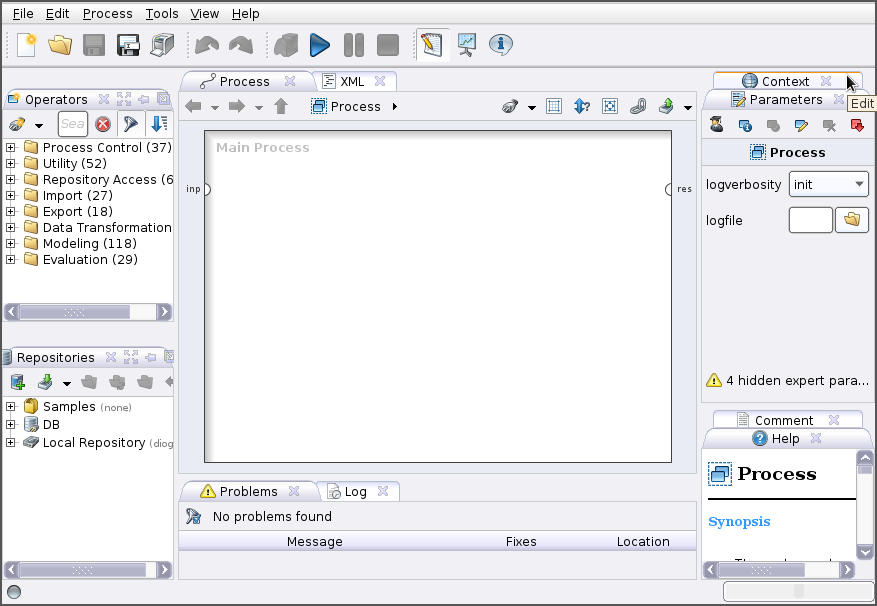
\includegraphics[width=0.6\textwidth]{rapidminer}
	\caption{RapidMiner's interface}
    \label{fig:rapidminer}
  \end{center}
\end{figure}

\subsubsection{WEKA}
Weka \footnote{WEKA: \url{http://www.cs.waikato.ac.nz/ml/weka/}} is an open source tool that collects several machine learning algorithms and allows its user to easily apply those algorithms to data mining tasks \cite{han2006data}. Created at the University of Waikato, New Zeland in 1997 (the current version was completely rewritten in 1997, despite the first iteration of the tool being developed as early as 1993), it's still in active development to date. Weka supports several common data mining tasks, like data preprocessing, classification, clustering, regression and data visualization. Its core libraries are written in Java and allow for an easy integration of its data mining algorithms in pre existing code and applications. Other than that, Weka can be used directly through a command line/terminal or through one of its multiple GUIs (Figure \ref{fig:weka}). Its simple API and well structure architecture allow it to be easily extended by users, should they need new functionalities.

\begin{figure}[htb]
  \begin{center}
    \leavevmode
    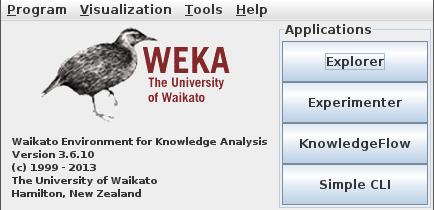
\includegraphics[width=0.6\textwidth]{weka}
	\caption{WEKA's interface}
    \label{fig:weka}
  \end{center}
\end{figure}

\subsubsection{R}
R \footnote{R: \url{http://www.r-project.org/}} is a free software environment for statistical computing and graphics. It compiles and runs on a wide variety of UNIX platforms, Windows and MacOS. R provides a wide variety of statistical (linear and nonlinear modeling, classical statistical tests, time-series analysis, classification, clustering, among others) and graphical techniques, and is highly extensible.  R is typically used by statisticians and data miners, either for direct data analysis or for developing new statistical software \cite{fox2005using}.\\
R is an open-source implementation of the S programming language, borrowing some characteristics from the Scheme programming language. Its core is written in a combination of C, Fortran and R itself. It is possible to directly manipulate R objects in languages like C, C++ and Java. R can be used directly through the command line or through several third party graphical user interfaces like Deducer \footnote{Deducer: http://www.deducer.org/pmwiki/index.php}. There are also R wrappers for several scripting languages.\\
R provides several different statistical and graphical techniques, including linear and nonlinear modeling, classical statistical tests, time-series analysis, classification, clustering, among others. It can also be used to produce publication-quality static graphics. Tools like Sweave \cite{leisch2002sweave} allow users to embed R code in \LaTeX documents, for complete data analysis.

\subsubsection*{arules}
The arules package \footnote{arules: \url{http://cran.r-project.org/web/packages/arules/index.html}} is a R package for mining association rules and frequent itemsets. Its sister package, arulesViz \footnote{http://cran.r-project.org/web/packages/arulesViz/index.html}, allows the visualization of the results found by arules. Since it is common to work with large sets of rules and itemsets, the package uses sparse matrix representations to minimize memory usage. The infrastructure provided by the package was also created to explicitly facilitate extensibility, both for interfacing new algorithms and for adding new types of interest measures and associations.

\subsubsection*{TraMineR}
TraMineR \footnote{TraMineR: \url{http://mephisto.unige.ch/traminer/}} (a contraction of Life Trajectory Miner for R) is a R-package for mining, describing and visualizing sequences of states or events, and more generally discrete sequential data. An example of the visualization features can be found in Figure \ref{fig:traminer}. Its primary aim is the analysis of biographical longitudinal data in the social sciences, such as data describing careers or family trajectories. Most of its features also apply, however, to non temporal data. TraMineR is developed at the Institute for Demographic and Life Course Studies (IDEMO), University of Geneva, Switzerland under the responsibility of the TraMineR Scientific Committee. 

\afterpage{
\begin{figure}[!htb]
  \begin{center}
    \leavevmode
    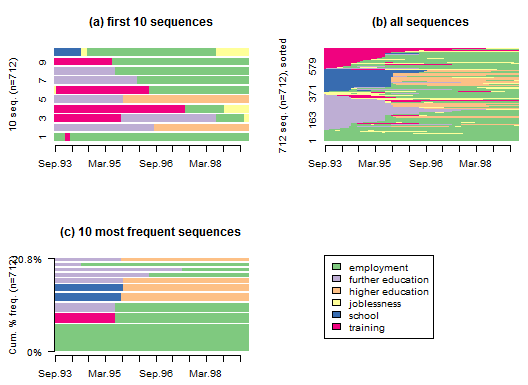
\includegraphics[width=0.8\textwidth]{traminer}
	\caption[An example of data visualization using TraMineR]{An example of data visualization using TraMineR\protect\footnotemark}
    \label{fig:traminer}
  \end{center}
\end{figure}
\footnotetext{Image extracted from: \url{http://mephisto.unige.ch/traminer/preview-visualizing.shtml}}
}

\subsubsection{SPMF (Sequential Pattern Mining Framework)}
SPMF \footnote{SPMF: \url{http://www.philippe-fournier-viger.com/spmf/}} is an open-source data mining library written in Java and distributed under the GPL v3 license. It includes implementations for sequential pattern mining, association rule mining, frequent itemset mining, sequential rule mining, and clustering algorithms, and has over 80 citations.

\section{Patterns}\label{sec:patterns}
User Interaction (UI) patterns are well-documented in a various number of sources \cite{tidwell2010designing,van2001patterns, neil12standard,sinnig2005patterns}. The patterns already supported (like the Search and Master/Detail patterns) enter the list of most popular patterns, according to the sources found, and if the selection of supported patterns were to be broadened, the pick of the next one(s) would be heavily influenced by the literature. Lin and Landay's approach \cite{lin2008employing} uses UI patterns for Web applications that run on PCs and mobile phones, and prompt-and-response style voice interfaces. Pontico \textit{et al.}'s approach \cite{pontico2008organizing} presents UI patterns common in eGovernment applications.

\section{Chapter Conclusions}
In this section we gave a brief introduction of concepts that serve as basis for this dissertation, namely reverse engineering and data mining, in specific association learning and its subtype, sequence pattern mining.

We also reviewed the state of the art on the following topics:
\begin{enumerate}
\item \textbf{Reverse engineering approaches}, subcategorized by approaches that extract information from execution traces, approaches that extract information from Web applications, and approaches that infer patterns from Web applications;
\item Popular \textbf{capture-replay tools};
\item Data mining \textbf{tools and frameworks};
\item UI \textbf{patterns}.
\end{enumerate}

At this moment we are still evaluating the best approach to follow regarding how we're going to analyze our data, since we are trying to find a method that efficiently evaluates all data produced by the PARADIGM-RE tool, and not just mine the execution traces.  As such, we presented ILP as an alternative approach for this situation. In case ILP techniques become in fact necessary, further work will include a more profound and complete
revision.
\chapter{RE-TOOL}\label{chap:approach}

\section*{}

%Este capítulo deve começar por fazer uma apresentação detalhada do problema a resolver\footnote{Na introdução a apresentação do problema foi breve.} podendo mesmo, caso se justifique, constituir-se um capítulo com essa finalidade.

%Deve depois dedicar-se à apresentação da solução sem detalhes de implementação. Dependendo do trabalho, pode ser uma descrição mais teórica, mais ``arquitetural'', etc.
In this chapter, we begin by giving a brief overview of PBGT, the research project the developed work is inserted in. Afterwards, the previous approach and current tool are broken down in components and explained in detail.

\section{PBGT Overview}\label{sec:pbgt}

As mentioned before, the focus of this dissertation is the reverse engineering component of a research project named PBGT (\textit{Pattern-based GUI Testing}) \cite{moreira2013pattern}. The goal of this project is to develop a model-based GUI testing approach and supporting tool, that can be used in industrial contexts.\\

\subsection{Architecture}
The PBGT supporting tool has main five components: 
\begin{enumerate}
\item \textbf{PARADIGM}, a DSL (\textit{Domain Specific Language}) to define GUI testing models based on UI Test Patterns \cite{enase14}; 
\item \textbf{PARADIGM-RE}, a Web application reverse engineering tool whose purpose is to extract UI patterns from Web pages without access to their source code, and use that information to generate a test model written in PARADIGM; 
\item \textbf{PARADIGM-ME}, a modeling and testing environment, built to support the creation of test models \cite{conf_icst_MonteiroP13}; 
\item  \textbf{PARADIGM-TG}, an automatic test case generation tool that generates test cases from test models defined in PARADIGM according to coverage criteria selected by the tester; 
\item and finally, a test case execution tool, named \textbf{PARADIGM-TE}, which executes test cases, analyzes their coverage with a coverage analysis tool named \textbf{PARADIGM-COV}\cite{vilela2014cov}, and returns detailed execution reports. 
\end{enumerate}

The architecture and workflow of the project is shown in Fig. \ref{fig:pbgt}.\\

\begin{figure}[!htb]
\centering
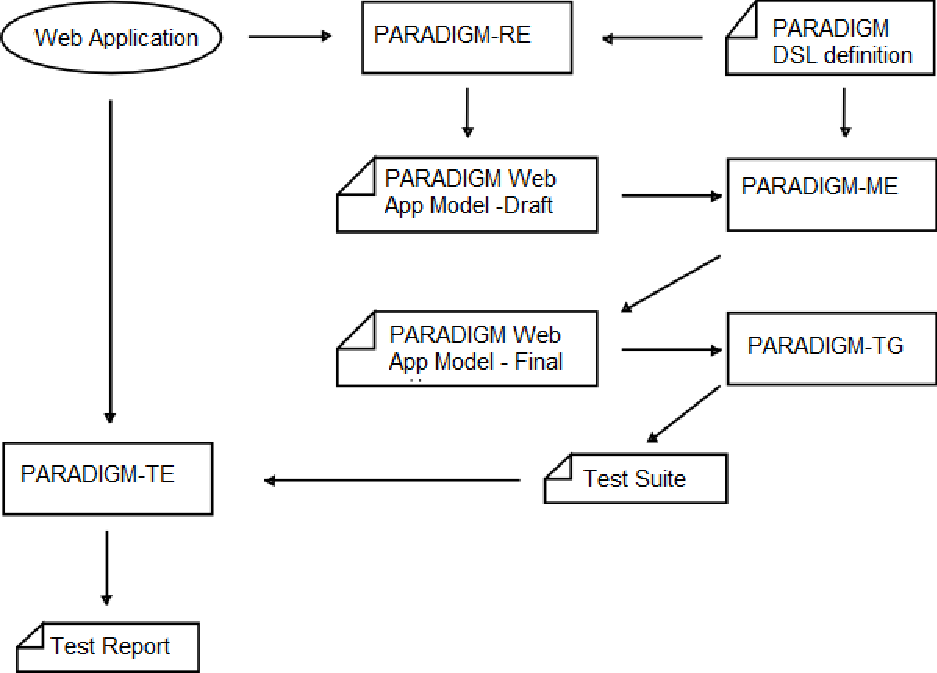
\includegraphics[width=\textwidth]{pbgt}
\caption{An overview of the PBGT project.}
\label{fig:pbgt}
\end{figure}

\subsection{PARADIGM DSL}\label{sec:dsl}
%falar doc conetores e, do init e do end, e falar também dos elementos estruturais: Form e Group

PARADIGM is a DSL to be used in the domain of PBGT. The goal of the language is to gather applicable domain abstractions (e.g., UI test patterns), allow specifying relations between them and also provide a way to structure the models in different levels of abstraction to cope with complexity. PARADIGM's meta-model is illustrated in Figure \ref{fig:dsl}.\\

\begin{figure}[!htb]
\centering
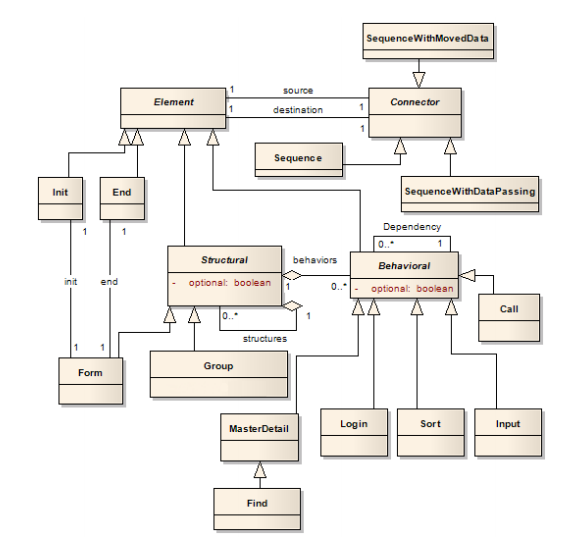
\includegraphics[width=\textwidth]{dsl}
\caption{PARADIGM DSL Meta-model.}
\label{fig:dsl}
\end{figure}

The PARADIGM language is comprised by elements and connectors \cite{moreira2013pattern}. There are four types of elements: \textit{Init} (to mark the beginning of a model), \textit{End} (to mark the termination of a model), \textit{Structural} (to structure the models in different levels of abstraction), and \textit{Behavioral} (UI Test Patterns describing the testing goals).\\

As models become larger, coping with their growing complexity forces the use of structuring techniques such as different hierarchical levels that allow use one entire model \textbf{A} inside another model \textbf{B} abstracting the details of \textbf{A} when within \textbf{B}. Structuring techniques are common in programming languages like C and Java, with constructs such as modules and classes. \textit{Form} is a structural element that may be used for that purpose. A \textit{Form} is a model (or sub-model) with an \textit{Init} and an \textit{End} elements. \textit{Group} is also a structural element but it does not have \textit{Init} and \textit{End} and, moreover, all elements inside the \textit{Group} are executed in an arbitrary order.\\

\begin{figure}[!htb]
\centering
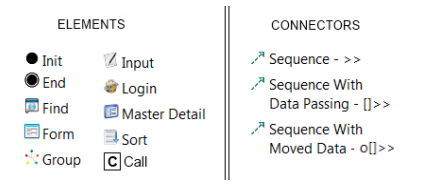
\includegraphics[width=0.5\textwidth]{dsl1}
\caption{PARADIGM syntax.}
\label{fig:dsl1}
\end{figure}

PARADIGM elements and connectors are described by: (i) an icon/figure to represent the element graphically and (ii) a short label to name the element. The overall syntax of the DSL is illustrated in Figure \ref{fig:dsl1}. Additionally, elements within a model have a number to identify them, and optional elements have a ``op" label next to its icon/figure.\\

This language has three connectors: \textit{Sequence}, \textit{SequenceWithDataPassing}, and \textit{SequenceWithMovedData}. \textit{Sequence} indicates that the testing strategy related to the target element cannot start until the testing strategy of the source element has completed. \textit{SequenceWithDataPassing} has the same meaning as \textit{Sequence}, and additionally indicates that the target element receives data from the source element. \textit{SequenceWithMovedData} has a similar meaning to \textit{SequenceWithDataPassing}, but the source element moves data to the target instead of transferring a copy. In addition, there is another kind of relation among elements -- \textit{Dependency} -- indicating that the target element depends on the properties of a set of source elements, for instance, when it is the result of a calculation. \\

\subsubsection{UITP (User Interface Test Patterns)}

A UI Test Pattern defines a test strategy to test a specific UI pattern, which is formally defined by a set of test goals (for later configuration)\cite{moreira2013pattern} with the form:

\begin{equation}< Goal; V; A; C; P >\end{equation}\label{eq:ui_}

\textit{Goal} is the \textit{ID} of the test. \textit{V} is a set of pairs { [\textit{variable}, \textit{inputData}] } relating test input data with the variables involved in the test. \textit{A} is the sequence of actions to perform during test case execution. \textit{C} is the set of possible checks to perform during test case execution, for example, “check if it remains in the same page”. \textit{P} is a Boolean expression (precondition) defining the set of states in which it is possible to execute the test. The language also defines language constraints to guarantee the building of well-formed models, such as ``\textit{A Connector cannot connect an element to itself}'' and ``\textit{A Connector cannot have Init as destination, or End as source}'', to cite a few examples.\\

The UI Patterns defined in the PARADIGM language are:
\begin{itemize}
\item \textbf{Login}: This pattern is commonly found in Web applications, especially in the ones that restrict access to functionalities or data. Usually consists of two input fields (a normal input box for email or username, and a cyphered text for the password) and a submit button, with optionally a ``remember me'' checkbox. The authentication process has two possible outcomes: valid and invalid. Upon authentication failure a message may be shown. 
\item \textbf{Find}: This pattern consists of one or more input fields, where the user inserts keywords to search, and a submit button to start the search. The search may be submitted via a submit button, or dynamically upon text insertion. When the search is successful, the website shows a list of results; upon failure, an error message may be shown.
\item \textbf{Sort}: This pattern sorts a list of data by a common attribute (e.g., price, name, relevance, etc.) according to a defined criteria (ascending or descending, alphabetically, etc.).
\item \textbf{Master Detail}: This pattern is present in a web page when selecting an element from a set (called \textit{master}) results in filtering/updating another related set (called \textit{detail}) accordingly. For example, clicking on a checkbox associated to a brand may include (or exclude) products of that brand in a product search result list. Generally the only elements changed are the elements belonging to the \textit{detail} set.
\item \textbf{Call}: This pattern is any kind of element where a click triggers some procedure that may result in a change of page.
\end{itemize}

\subsection{Produced Models}

The models produced by the reverse engineering tool PARADIGM-RE consist of a XML file in the format required by the PARADIGM-ME which contains information about the UI Test Patterns needed to test the UI Patterns found: their name, the input values for their variables, i.e., the values used during the exploration process, and blank pre-conditions and checks for the tester to fill in. The UI Test Patterns within the model are connected in a linear path according to the exploration order. The testing configuration information needs to be complemented and validated by the tester afterwards in order to generate test cases and execute them over the web application under analysis.

\section{Reverse Engineering Approach}\label{sec:re}

\subsection{Previous Tool}\label{sec:prev}

The  approach described in this dissertation aims to improve on the previous work \cite{nabuco2013inferring} done on the PARADIGM-RE tool. In particular it aims to be fully automatic. The previous tool required the intervention of the user to interact with the web application under analysis in order to save the interaction traces and proceed from there. It extracted information from an user's interaction with the Web application under analysis, analyzed the information, produced some metrics (such as the total ratio of the LOC (\textit{lines of code}), length of all visited pages and the ratio of two subsequent pages), and finally used those metrics and the user interaction's information to infer UI patterns via a set of heuristic rules. \\
This tool identifies interface patterns using Machine Learning inference with the Aleph ILP system \footnote{Aleph: \url{http://www.cs.ox.ac.uk/activities/machlearn/Aleph/aleph\_toc.html}} running on user interaction execution traces produced using Selenium \footnote{Selenium: \url{http://docs.seleniumhq.org/}}. It was deemed necessary then to transform the whole process into an iterative one, with the model being updated at every iteration. 

This was accomplished in \cite{nabuco2014inferring}, where the tool was extended with a pattern identifying module using heuristics. The structure of the previous tool can be seen in Figure \ref{fig:retool_prev}. 

\begin{figure}[!htb]
 \begin{center}
 \leavevmode
 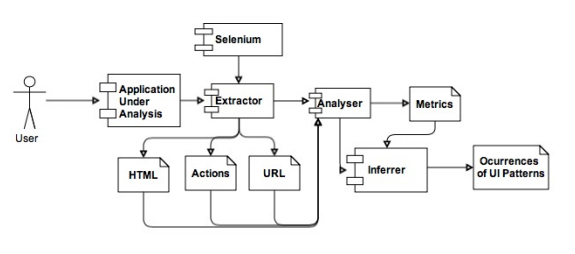
\includegraphics[width=\textwidth]{retool_prev}
 	\caption[Structure of the PARADIGM-RE tool]{Structure of the PARADIGM-RE tool \cite{nabuco2014inferring}}
 	\label{fig:retool_prev}
 \end{center}
\end{figure}

The user interacts with the Web application, using Selenium to save the actions taken. An example of execution traces saved by Selenium can be seen on table \ref{tab:amazontraces}. 

\begin{table}[!htb]
\begin{tabular}{|l|l|l|}
\hline
\multicolumn{3}{|c|}{\textbf{amazon}} \\ \hline
\textbf{actionType} & \textbf{element} & \textbf{text} \\ \hline
open & / & \\ \hline
type & id=twotabsearchtextbox & tablet \\ \hline
clickAndWait & css=input.nav-submit-input & \\ \hline
select & id=sort & label=Most Popular \\ \hline
click & id=pagnNextString & \\ \hline
click & id=pagnPrevString & \\ \hline
clickAndWait & link=Image & \\ \hline
clickAndWait & link=Detail & \\ \hline
click & link=android tablet & \\ \hline
click & css=li.refinementImage \textgreater a.. \textgreater span.refinementLink & \\ \hline
clickAndWait & css=\#result\_3 \textgreater h3.newaps \textgreater a \textgreater span.lrg.bold & \\ \hline
clickAndWait & link=Explore similar items & \\ \hline
\end{tabular}
\caption[An example of execution traces produced on the Amazon.com website, extracted using Selenium IDE.]{An example of execution traces produced on the Amazon.com website, extracted using Selenium IDE\protect\footnotemark.}
\label{tab:amazontraces}
\footnotetext{Selenium IDE: \url{http://docs.seleniumhq.org/}}
\end{table}

The \textbf{extractor} saves the HTML of all pages visited, their URLs, and the actions taken in each page. All that information is passed along to the \textbf{analyzer}, whose purpose is to produce metrics like page ratios, differences between consecutive pages, and others, from the data given. Those metrics are passed to the \textbf{inferrer}, who runs the heuristics suite, identifies existing patterns, and produces a XMI file with the occurrences found. An example of the contents of such a file, with one of each inferrable pattern, can be found on Listing \ref{lst:paradigm}.

\lstset{language=XML,caption={An example of a .paradigm file with identified patterns},label=lst:paradigm}
\begin{lstlisting}
<?xml version="1.0" encoding="UTF-8"?>
<Paradigm:Model xmi:version="2.0" xmlns:xmi="http://www.omg.org/XMI"
 xmlns:Paradigm="http://www.example.org/Paradigm" title="patterns"/>
	<nodes xsi:type="Paradigm:Init" name="XInit" number="1"/>
	<nodes xsi:type="Paradigm:Sort" name="Sort2" number="2"/>
    <nodes xsi:type="Paradigm:Login" name="Login3" number="3"/>
    <nodes xsi:type="Paradigm:MasterDetail" name="MasterDetail4" number="4"/>
    <nodes xsi:type="Paradigm:Input" name="Input5" number="5"/>
    <nodes xsi:type="Paradigm:Find" name="Find6" number="7"/>
	<nodes xsi:type="Paradigm:End" name="End" number="8"/>
</Paradigm:Model>
\end{lstlisting}

This approach was evaluated on several worldwide used Web applications and the results were deemed satisfactory, since the tool identified most of the occurring patterns and their location on the page. However, there are some patterns the tool doesn't identify, such as the Menu pattern, and the high number of false positive results indicate the heuristics are considered to be still in an incipient state.

The information saved from a user interaction was the source code and URLs of the visited pages, and the interaction's execution trace. An execution trace is the sequence of user actions executed during the interaction with a software system, such as clicks, text inputs and also some information of the system state (e.g., the information that is being displayed). An example of an execution trace file used by the tool can be seen in Table \ref{tab:exec}.\\

\begin{table}[!htb]
\resizebox{0.9\textwidth}{!}{
  \begin{tabular}{| c | c | c |}
     \hline
     \textbf{Action} & \textbf{Target} & \textbf{Value} \\ \hline
     type&id=input\_username &``user1" \\ \hline
     type&id=input\_password &``123pass" \\ \hline
     clickAndWait & css=input[type=``submit"]&EMPTY \\
     \hline
     type&id=searchInput&``coffee" \\ \hline
	 clickAndWait & id=mw-searchButton&EMPTY\\
     \hline
     select&id=sort&label=Price:Low to High \\
     \hline
     %%%%%
     click&id=collapseButton1&EMPTY\\\hline
     click&link=Next&EMPTY\\\hline
     typeAndWait&id=freeSearch&ministry\\\hline
     type&id=authcode&T75Y5\\\hline
     type&name=firstName&james\\\hline
	 type&name=lastName&bond\\\hline
     click&//ul[@id='ref1']/li[5]/a/span&EMPTY\\\hline
  	 \end{tabular}
}
\caption{Abbreviated example of an execution trace file.}
\label{tab:exec}
\end{table}

The previous reverse engineering approach identified the \textit{Find}, \textit{Login}, \textit{Sort}, \textit{Input} and \textit{MasterDetail} patterns, and produced a high number of false positives \cite{nabuco2013inferring}. Additionally, and as already mentioned, the exploration process was done by saving the user interaction with the Web application under test, requiring human interaction to identify patterns. The results were dependent on the execution traces followed by the tester. \\

\subsection{Current Tool}

The work described in this dissertation is a completely new tool, unrelated to the previous tool, but which has the same primary aim as the previous tool (to identify UI patterns in the Application Under Test (AUT)), only with other goals. The first is to remove the need for user interaction with the AUT to identify patterns, by providing a reverse engineering process to explore automatically the web application under analysis. The second is to refine and improve the pattern inferring process, and lower or eliminate completely the percentage of false positives. The third is to identify more patterns than the previous tool (including patterns that are going to be included in latter versions of the PARADIGM DSL, like the Menu pattern).\\

The architecture of the tool is seen in Figure \ref{fig:retool}.
\begin{figure}[!htb]
\centering
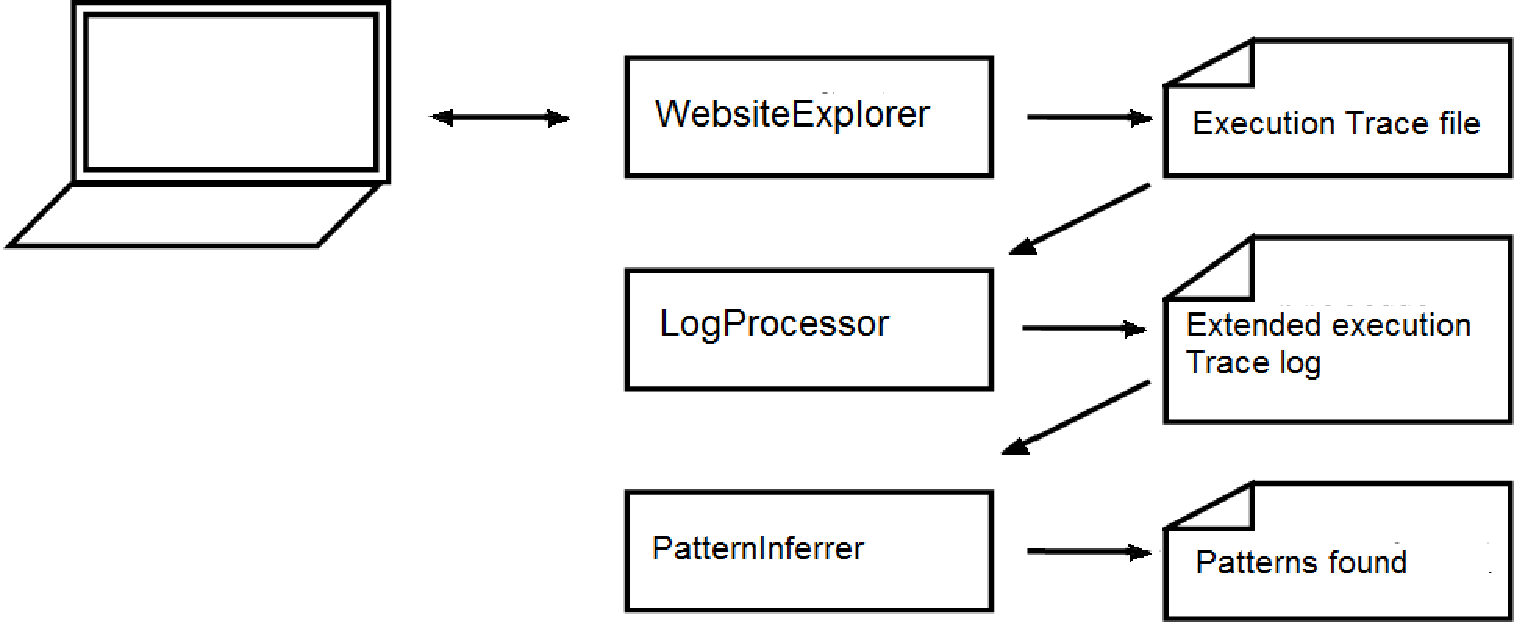
\includegraphics[width=\textwidth]{retool}
\caption{The architecture of the approach.}
\label{fig:retool}
\end{figure}

The approach can be divided into three parts: \textbf{WebsiteExplorer}, \textbf{LogProcessor}, and \textbf{PatternInferrer}.

\textbf{WebsiteExplorer} loads user configurations (more details on Section \ref{sec:conf}), interacts automatically with the AUT and produces an execution trace file with the actions taken (see Table \ref{tab:exec} for an example). \textbf{LogProcessor} is a text parser. It analyzes the previous file, parses each line, searches for important keywords and uses them to identify the action contained in the line, and produces an updated execution trace file (see Table \ref{tab:exec1} for an example). Finally, \textbf{PatternInferrer} analyzes the updated execution file, identifies the existent patterns, their location in the website and any existing parameters, and produces an XML file with the results. The patterns identifiable by this tool are all of those defined in the PARADIGM language, plus the \textit{Menu} UI pattern, which is going to be included in the PARADIGM DSL in the future. \\

\subsubsection{AUT Exploration (WebsiteExplorer)}\label{sec:inter}
The interaction process is described in a simplified manner in Algorithm \ref{alg:seeker}.

\begin{algorithm}
  %\SetLine
  \KwData{number\_of\_actions, number\_of\_iterations, website\_base\_url, configuration\_file}
  \KwResult{execution\_trace\_file}
  
  current\_action := 0; redirections := 0\;
  configuration := parseConfigurationFile()\;
  
  \While{current\_action $<$ configuration.number\_of\_actions}{
    \If{configurations.isSearchingForMenu()}
      {
        menuElements.add(getMenuElementsInPage())\;
      }
    \If{configuration.isSearchingForMasterDetail()}
    {
      masterElements.add(getMasterElementsInPage())\;
      detailElements.add(getDetailElementsInPage())\;
    }
  
  	list := extractValidNonVisitedElements\;
    next\_element := chooseNextElement(list)\;
  \eIf{next\_element == null}
  {%then
  	redirections++\;
    \eIf{redirection $<$ configuration.number\_of\_iterations}
    	{%then
        	go\_to\_base\_URL\;
            write\_to\_execution\_trace\_file\;
        }
        {%else
        	end\_program\;
        }
  }
  {%else
  	visit(element)\;
    visitedElements.add(element)\;
    write\_to\_execution\_trace\_file\;
    current\_action++;
    wait(configuration.politenessDelay)\;
  }
}

\caption{Pseudo-code algorithm to explore a page.}\label{alg:seeker}
\end{algorithm}

Currently the elements explored are \textit{$<$select$>$} elements, \textit{$<$input$>$} elements, and \textit{$<$a$>$} (link) elements. The way each element is visited is different: link elements are clicked; input elements get text (either a keyword or a number, depending on the type of input) and the containing form is submitted; and in the case of dropdown menus, a random option is selected and the surrounding form is submitted. The exception to the \textit{input} rule is when the element is identified as a \textit{login} element, in which case all the sibling elements (elements inside the form where the selected element is located) get text and only then the form is submitted.\\

Information about these elements is extracted via XPath\footnote{XPath: \url{www.w3schools.com/XPath/}}. Before interacting with an element, the algorithm makes the following checks: if the element has not been visited in the current page, and if the element contains any unwelcome keywords that if explored may drive the explorer into unwanted paths. These keywords may be general to all elements (anything that edits information or contains the words 'buy'/'sell', for example, that would lead to purchase products) or element-specific (input elements cannot contain the attribute '\textit{disabled}' or'\textit{readonly}', if they are to be interacted with). All elements have the same probability of being chosen from a list of elements.\\

The execution trace file produced is a CSV (\textit{Comma-separated values}) file with three columns: \textbf{action}, the type of action executed (\textit{click, type}, or \textit{select} when selecting an option in a dropdown menu -- it may also contain the suffix \textit{AndWait}, which indicates a page change); \textbf{target}, the identifier of the visited element; and \textbf{value}, which has the parameter for the action and may be empty (for example, in the case of \textit{type} actions, it is the inserted text). An example of a produced CSV file can be seen in Table ~\ref{tab:fullexec}, in Section \ref{sec:appendix}.\\

The exceptions are the Menu and MasterDetail patterns. Since the explorer cannot be relied on to explore every element belonging to these patterns in each page, elements belonging to these patterns are found through analyzing the current page source and extracting all elements that obey a set of rules. For the Menu pattern, the anchor links that are in \textit{$<$nav$>$}, \textit{$<$header$>$} or \textit{$<$footer$>$} tags are automatically included as part of the Menu pattern. Besides this, Menu elements and Master Detail are identified by a set of identifiers passed via the configuration file, and they are identified as its respective pattern if they respect the condition \texttt{(//*[contains(@class,identifier)] OR //*[contains(@id,identifier)] OR //*[contains(@name,identifier)])}.\\

The results of the HTML analysis are passed directly to the \textbf{PatternInferrer} to be written in the final output file (see Section \ref{sec:inf}).\\

\subsubsection{Configuration}\label{sec:conf}
To improve results, almost all components used in the website interaction and pattern identifying processes can be loaded to the application via a XML configuration file, the only exception being the PatternInferrer grammar. This is done to allow the maximum flexibility to the tester to adjust the tool to the web application to test.\\

The components and values that can be loaded via configuration file are: 
\begin{itemize}
\item[] \textbf{actions}: number of actions the crawler will execute before stopping;
\item[] \textbf{redirections}: number of redirects to the home page the crawler will do before stopping; 
\item[] \textbf{politenessDelay}: time to wait (in milliseconds) after each action;
\item[] \textbf{typedKeywords}: list of words to insert in text input elements;
\item[] \textbf{searchKeywords}: regex with keywords that identify search elements;
\item[] \textbf{sortKeywords}: regex with keywords that identify sort elements;
\item[] \textbf{loginKeywords}: regex with keywords that identify login elements;
\item[] \textbf{generalWordsToExclude}: regex with keywords that mark elements that should not be accessed;
\item[] \textbf{menuIdentifiers}: list of ids/classes/names that identify menu elements;
\item[] \textbf{masterIdentifiers}: list of ids/classes/names that identify master elements;
\item[] \textbf{detailIdentifiers}: list of ids/classes/names that identify detail elements;
\item[] \textbf{historyFilepath}: specify absolute file path for history file;
\item[] \textbf{processedHistoryFilepath}: specify absolute file path for processed history file;
\item[] \textbf{patternsFilepath}: specify absolute file path for PARADIGM model file;
\item[] \textbf{patternsToFind}: list of patterns that the explorer can search for - if "all" occurs, there will be no restriction;
\item[] \textbf{loginConfiguration}: credentials for a correct login in the web app;		
\item[] \textbf{tokenizerPatterns}: patterns for LogProcessor;
\item[] \textbf{includeChildrenNodesOnInteraction}: boolean; on interaction with an input or select element, if children elements should be included  in the history file, but not interacted with;
\end{itemize}

\subsubsection{Action File Processing (LogProcessor)}\label{sec:fp}

This component is a lexical analyzer, whose role is to examine the execution trace file line by line and identify the type of each action written therein. It has a data structure (which serves as its lexical grammar) containing the rules it is going to search for, and each has the following attributes: \textbf{pattern\_name}, the identifier for the rule; \textbf{identifying\_regex}, and a regex (Regular Expression\footnote{Regex: \url{http://www.regular-expressions.info/}}) that identifies an action of that type. \\

For every line, not all rules are tested; if a rule matches the line, first a camel-case token (composed by the sum of the action type and the rule's name) is produced, added to the processed trace file, and then the program moves on to the next line. If no rules match, only the action is written on the file. An example of file processing may be seen in Table \ref{tab:exec}.\\

\begin{table}[!htb]
\resizebox{0.9\textwidth}{!}{
  \begin{tabular}{| c | c | c || c |}
     \hline
     \textbf{Action} & \textbf{Target} & \textbf{Value} & \textbf{Processing Return} \\ \hline
     type&id=input\_username &user1&typeUsername \\ \hline
     type&id=input\_password &123pass&typePassword \\ \hline
     clickAndWait & css=input&EMPTY&clickFormSubmit \\
      & [type=``submit"] & & PageChange\\
     \hline
     type&id=searchInput&coffee&typeSearch \\ \hline
	 clickAndWait & id=mw-searchButton&EMPTY&clickSearch\\
      & & & PageChange \\ \hline
     select&id=sort&label=Price: &selectSort \\
      & & Low to High& \\
     \hline
     %%%%%%
     click&id=collapseButton1&EMPTY&clickCollapse\\ \hline
     click&link=Next&EMPTY&clickNextLink \\ \hline
     typeAndWait&id=freeSearch&ministry&typeSearch \\
      & & & PageChange \\ \hline
     type&id=authcode&T75Y5&typeAuth\\\hline
     type&name=firstName&james&typeFirstName\\\hline
	 type&name=lastName&bond&typeLastName\\\hline
     click&//ul[@id='ref\_679781011']/li[5]/a/span&EMPTY&click\\\hline
  	 \end{tabular}
} 
\caption{Example of an execution trace file, and of processed lines.}
\label{tab:exec1}
\end{table}

The identifiable tokens by default are: \textit{login, username, email, password, verifyPassword, submit, captcha, auth, search, sort, link, option, checkbox, radio, homeLink, imageLink, nextLink, prevLink, firstLink, lastLink, languageLink, buttonLink, searchResultLink, link, collapse, firstNameInput, lastNameInput, numberInput, input, button}, and \textit{clear}. However, the identifiable patterns can also be overridden and added to via a configuration file (see Section \ref{sec:conf}).\\

The tokens produced by the LogProcessor affect the pattern inferring done by PatternInferrer. For example, the patterns involved in the inferring of the Login pattern are \textit{username, email, login} (these identify username and email inputs, and login inputs or actions, depending on which action the token is appended to), \textit{password} (which identifies a password input),  and \textit{submit}, which are used to indicate the closing of a classical form submit action (when \textit{matchSubmit(line)} is true), and thus, the end of a standard pattern. Some patterns are identified to distinguish between proper patterns and other types of action non relevant to the inferring process, such as \textit{verifyPassword}, which can be used to distinguish between a Login form and a Register form, and \textit{searchResultLink}, which prevents search result links from being marked as part of a Find pattern. Some exist simply to give better context to the action, like \textit{nextLink} or \textit{lastName}. An example of a processed execution trace file (resulting of running LogProcessor on the contents of Table \ref{tab:fullexec}) can be seen in Listing \ref{lst:full_exec_proc}.\\

\subsubsection{UI Pattern Inferring (PatternInferrer)}\label{sec:inf}

This component is a syntactical analyzer, that takes as input the extended execution trace file returned by the \textit{LogProcessor}, runs it against a predefined grammar, and returns the patterns found. The processing rules are formalized in Table \ref{tab:grammar}.

\begin{table}[!htb]
\begin{tabular}{rcl}
  $\bnfpn{pattern}$ & $\bnfpo$ & $\bnfpn{login}$ $\bnfor$ $\bnfpn{find}$ $\bnfor$ $\bnfpn{sort}$ $\bnfor$ $\bnfpn{input}$ $\bnfor$ $\bnfpn{call}$ \\
  
  $\bnfpn{find}$  & $\bnfpo$ &  $\bnfpn{match-find}$ $\bnfsp$ $\bnfpn{opt-submit}$ \\
  
  $\bnfpn{sort}$ & $\bnfpo$ &  $\bnfpn{match-sort}$ $\bnfsp$ $\bnfpn{opt-submit}$ \\
  
  $\bnfpn{input}$ & $\bnfpo$ &  $\bnfpn{match-input}$ $\bnfsp$ $\bnfpn{opt-submit}$ \\
  
  $\bnfpn{call}$ & $\bnfpo$ &  $\bnfpn{match-link}$ $\bnfsp$ $\texttt{PageChange}$ \\
  
  $\bnfpn{login}$ & $\bnfpo$ &  $\bnfpn{opt-login-rec}$ $\bnfsp$ $\bnfpn{match-user-pass}$\\
  & & $\bnfsp$ $\bnfpn{match-submit}$ \\
  
  $\bnfpn{match-user-pass}$ & $\bnfpo$ &  $\bnfpn{match-user}$ $\bnfsp$ $\bnfpn{match-pass}$ \\
  & & $\bnfor$ $\bnfpn{match-pass}$ $\bnfsp$ $\bnfpn{match-user}$ \\
  
  $\bnfpn{opt-submit}$ & $\bnfpo$ &  $\bnfpn{match-submit}$ $\bnfor$ $\bnfes$ \\
  
  $\bnfpn{match-submit}$ & $\bnfpo$ &  $\texttt{clickFormSubmit}$ $\bnfor$ $\texttt{clickButton}$ \\
  
  $\bnfpn{match-find}$ & $\bnfpo$ &  $\bnfpn{opt-find-rec}$ $\bnfsp$ $\bnfpn{search-item}$ $\bnfsp$ $\bnfpn{opt-find-rec}$ \\
  
  $\bnfpn{match-sort}$ & $\bnfpo$ &  $\texttt{clickSort}$ $\bnfor$ $\texttt{selectSort}$ \\
  
  $\bnfpn{match-input}$ & $\bnfpo$ &  $\texttt{clickInput}$ $\bnfor$ $\texttt{typeInput}$ \\
  & & $\bnfor$ $\texttt{typeNumberInput}$ \\ 
  & & $\bnfor$ $\texttt{typeFirstNameInput}$ \\
  & & $\bnfor$ $\texttt{typeLastNameInput}$ \\
  
  $\bnfpn{match-user}$ & $\bnfpo$ &  $\bnfpn{opt-login-rec}$ $\bnfsp$ $\bnfpn{user}$ $\bnfsp$ $\bnfpn{opt-login-rec}$ \\
  
  $\bnfpn{match-pass}$ & $\bnfpo$ &  $\bnfpn{opt-login-rec}$ $\bnfsp$ $\bnfpn{pass}$ $\bnfsp$ $\bnfpn{opt-login-rec}$ \\
  
  $\bnfpn{user}$ & $\bnfpo$ &  $\texttt{typeUsername}$ \\
  & & $\bnfor$ $\texttt{typeEmail}$ $\bnfor$ $\texttt{typeLogin}$ \\
  
  $\bnfpn{pass}$ & $\bnfpo$ &  $\texttt{typePassword}$ \\
  
  $\bnfpn{match-opt-login}$ & $\bnfpo$ &  $\texttt{clickLogin}$ $\bnfsp$ $\texttt{PageChange}$ \\
  & & $\bnfor$ $\texttt{typeAuth}$ $\bnfor$ $\texttt{typeCaptcha}$ \\
  & & $\bnfor$ $\texttt{clickOption}$ $\bnfor$ $\texttt{clickRadio}$ \\
  
  $\bnfpn{match-link}$ & $\bnfpo$ &  $\texttt{clickLink}$ \\
   & & $\bnfor$ $\texttt{clickHomeLink}$ \\
   & & $\bnfor$ $\texttt{clickImageLink}$ \\
   & & $\bnfor$ $\texttt{clickNextLink}$ \\
   & & $\bnfor$ $\texttt{clickPrevLink}$ \\
   & & $\bnfor$ $\texttt{clickFirstLink}$ \\
   & & $\bnfor$ $\texttt{clickLastLink}$ \\
   & & $\bnfor$ $\texttt{clickLanguageLink}$ \\
   & & $\bnfor$ $\texttt{clickButtonLink}$ \\
   & & $\bnfor$ $\texttt{clickSearchResultLink}$ \\
  
  $\bnfpn{opt-find-rec}$ & $\bnfpo$ &  $\bnfpn{opt-find-rec}$ $\bnfor$ $\bnfpn{opt-search}$ \\
  & & $\bnfor$ $\bnfpn{search-item}$ $\bnfor$ $\bnfes$ \\
  
  $\bnfpn{opt-search}$ & $\bnfpo$ &  $\texttt{clickSearch}$ \\
  
  $\bnfpn{search-item}$ & $\bnfpo$ &  $\texttt{typeSearch}$ $\bnfor$ $\texttt{selectSearch}$ \\
  
  $\bnfpn{opt-login-rec}$ & $\bnfpo$ &  $\bnfpn{opt-login-rec}$ $\bnfor$ $\bnfpn{match-opt-login}$ $\bnfor$ $\bnfes$ \\
  & & \\
  \end{tabular}
%\end{bnf*}
\caption{Default grammar used by LogProcessor to tokenize the execution trace file ($\epsilon$ indicates an empty string).}
\label{tab:grammar}
\end{table}

If during the process the tool detects the same UI Pattern instance several times, the tool is capable of ignoring the repetitions. Its reasoning is explained in Figure \ref{fig:inferrer}.\\

\begin{figure}[!htb]
\centering
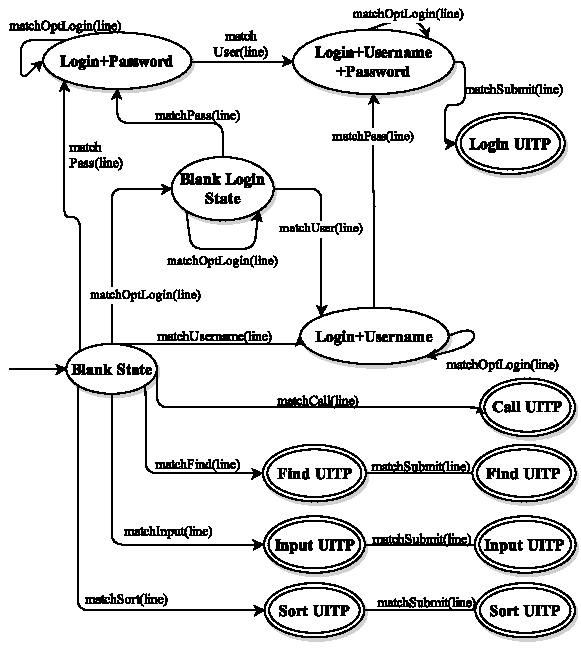
\includegraphics[width=\textwidth]{Global_State_Machine.pdf}
\caption{The inferrer's reasoning algorithm, expressed in a finite state machine.}
\label{fig:inferrer}
\end{figure}

For simplicity's sake, only the valid paths are shown in the figure (Fig. \ref{fig:inferrer}). All patterns except \textit{Login} can be valid even in the absence of a form submit action; this is done to account for dynamic submission via Javascript. In the case of the Login pattern, there can only be one password and one username or email record; this is done to distinguish login forms from register forms and password/email change forms.\\

The previous figure (Fig. \ref{fig:inferrer}) does not account for the \textit{Menu} and \textit{Master Detail} patterns; as mentioned before, these patterns are identified through HTML analysis and passed directly from the \textit{WebsiteExplorer} to the \textit{PatternInferrer} to write. This grammar only deals with the patterns identifiable through the execution trace file.\\

After the file is processed, an XMI file is produced containing all the pattern occurrences found, and the values assigned to each variable, as per Formula \ref{eq:ui_}. As mentioned before, the checks to perform within each test strategy and any preconditions must be specified by the tester later on in the PARADIGM-ME tool.\\

An example of a execution trace file extract from which a Login pattern can be inferred can be seen in Table \ref{tab:fullpattern}, and full example of a PARADIGM file (with inputs being  the contents of Table \ref{tab:fullexec} and Listing \ref{lst:full_exec_proc}) can be seen on Listing \ref{lst:full_pattern}.

\begin{table}[!htb]
\resizebox{0.9\textwidth}{!}{
\begin{tabular}{|c|c|c|c|}
\hline
\textbf{Action} & \textbf{Target} & \textbf{Value} & \textbf{Processing Return} \\ \hline
 & //a[@class=active &	 &  \\
clickAndWait & and @href=\ldots & EMPTY & clickLogin pageChange\\
&  and contains(text(),'Login')] & &  \\\hline
 & //input[@id=email & &  \\
type&  and @name=email & login@en.pt  & typeEmail\\
&  and @type=text] & & \\\hline
 & //input[@id=password  & &  \\
type& and @type=password & pass & typePassword\\
& and @name=password] & & \\\hline
 & //input[@id=save\_login &  &   \\
click& and @name=save\_login & EMPTY & clickLogin\\
&  and @type=checkbox] & & \\\hline
 & //input[@class=btn\_small grey &  &  \\
clickAndWait& and @name=commit & EMPTY & clickSubmit pageChange \\
&  and @type=submit] & & \\\hline
\end{tabular}
}
\caption{Execution trace example from which a Login pattern can be inferred.}
\label{tab:fullpattern}
\end{table}

\subsubsection{PARADIGM files produced by PatternInferrer}
The final PARADIGM files produced contain instances of UI Test Patterns, that correspond to all of the patterns discovered during the exploration made by the WebsiteExplorer and contain blank test configurations meant for the tester to fill in. The files are XMI files which follow the PARADIGM DSL (see Section \ref{sec:dsl}).

Each pattern is stored in a $<$\textit{nodes}$>$ tag, which has the following attributes: \textit{type} (the type of pattern), \textit{name} (a unique string identifier), \textit{number} (a unique integer identifier), \textit{incomingLinks} (the incoming sequence connector) and \textit{outgoingLinks} (the outgoing sequence connector).

Each $<$\textit{nodes}$>$ tag has two types of children: $<$\textit{configurations}$>$ tags, which contain testing configurations, and $<$\textit{fields}$>$ tags, which identify web elements involved in the testing configurations. Configurations are defined by attributes, and the specification of the test (such as data to insert or element to choose) are defined in $<$\textit{fields}$>$ child nodes. Some of the attributes that a configuration may have are: \textit{validity} (whether the inserted data is supposed to be valid or not); \textit{check} (the type of check to apply to the result of the operation); \textit{result} (the number of results expected - for testing Find patterns); \textit{master} (identifies the master in a MasterDetail pattern); and \textit{mappingURL} (the URL in which the testing elements are).

A simplified example of a generated model can be seen in Listing \ref{lst:paradigm_model}, in the Appendix chapter (Section \ref{sec:appendix}), and the corresponding graphic model, generated via PARADIGM-ME, can be seen in Figure \ref{fig:pbgt-me}.

\begin{figure}[!htb]
\centering
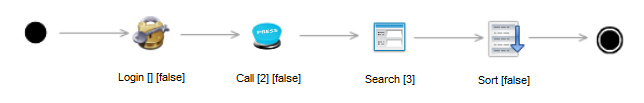
\includegraphics[width=\textwidth]{pbgt-me.png}
\caption{A simplified example of a generated model.}
\label{fig:pbgt-me}
\end{figure}

\section{Chapter Conclusions}
In this chapter we gave a brief overview of PGBT, explained in detail the previous and current tool, to better highlight their differences and explain their functioning. The previous tool requires user interaction to explore a Web application, analyzes the execution trace file, HTML source and URLs  of all pages visited, and infers patterns through a set of heuristic rules; the current tool is fully automatic, requires only the execution trace file, and infers patterns through syntactical analysis of a previously tokenized execution trace file.

\chapter{Case Study}\label{chap:validation}

In this chapter we introduce a case study, done to validate the developed work and assess its efficacy and compliance of the dissertation goals. 

\section{Evaluation}\label{sec:eval}

\subsection{Research Questions}

In order to evaluate the developed reverse engineering approach, some experiments were performed. They aimed to answer the following research questions:

\begin{itemize}
  \item[R1)] Is it possible to infer automatically UI Patterns from a Web application?\\
  \item[R2)] Is it possible to improve the results provided by the previous RE tool?\\
\end{itemize}

\subsection{Evaluation Results}

The RE tool was initially tested iteratively over a set of Web applications, with the goal of fine-tuning the inferring grammars used to discover UI Patterns.

Afterwards, the RE tool was used to detect UI Patterns in several widely used Web applications. This time, the purpose was to evaluate the RE tool, i.e., to determine which UI pattern occurrences the tool was able to detect in each application execution trace (ET), and compare them to the list of known to exist patterns.

Five applications were chosen from the most popular websites
\footnote{according to: \protect\url{http://en.wikipedia.org/wiki/List_of_most_popular_websites}}: Amazon, Wikipedia, Ebay, Youtube, Facebook and Yahoo.

The results of the experiments are presented in table \ref{tab:eval_curr}. This table shows the number of instances of each UI pattern that exist in the execution traces, the ones that the tools correctly found and the ones that the tools mistakenly found (false positives). In the case of the previous tool, the Menu and Call patterns weren't included because the tool doesn't identify those patterns.

\begin{table}[!htb]
\centering
\resizebox{0.9\textwidth}{!}{
  \begin{tabular}{| c | c | c | c | c |}
  \hline \multicolumn{5}{|c|}{\textbf{Previous Tool}} \\ \hline
     \textbf{Pattern} & \textbf{Present} & \textbf{True} & \textbf{False} & \textbf{False} \\
       & \textbf{in ET} & \textbf{Positive} & \textbf{Negative} & \textbf{Positive} \\ \hline
     Find & 15 & 9 & 6 & 0 \\
     Login & 4 & 3 & 1 & 0 \\
     Sort &  1 & 1 & 1 & 306 \\
     Input & 29 & 29 & 0 & 6 \\
MasterDetail & 58 & 58 & 0 & 22 \\ \hline
\textbf{Total} & \textbf{107 (100\%)} & \textbf{100 (93.46\%)} & \textbf{7 (6.54\%)} & \textbf{334 (312.15\%)} \\ \hline
    \hline \multicolumn{5}{|c|}{\textbf{Current Tool}} \\ \hline
     \textbf{Pattern} & \textbf{Present} & \textbf{True} & \textbf{False} & \textbf{False} \\
       & \textbf{in ET} & \textbf{Positive} & \textbf{Negative} & \textbf{Positive} \\ \hline
     Find & 15 & 13 & 2 & 0 \\
     Login & 4 & 4 & 0 & 0 \\
     Sort & 1 & 1 & 0 & 0 \\
     Input & 29 & 28 & 1 & 0 \\
     Call & 249 & 235 & 14 & 0 \\ 
     Menu & 212 & 212 & 0 & 4 \\
MasterDetail & 58 & 46 & 12 & 0 \\ \hline
\textbf{Total} & \textbf{568 (100\%)} & \textbf{539 (94.89\%)} & \textbf{29 (5.11\%)} & \textbf{4 (0.7\%)} \\ \hline
  \end{tabular}
}
\caption{Evaluation set results from the previous and current tool, given the same input.}
\label{tab:eval_curr}
\end{table}

As we can see in Table \ref{tab:eval_curr}, the current reverse engineering tool found few false positives, most related to the Menu UI Pattern. In addition it is worth to mention that the tool found 95.59\% of the  patterns present in the automatically explored execution traces. Given the same input, the current tool improved all of the statistics, and specially the rate of false positives.

However, the case study does not mention how many patterns were present in the web applications that were not visited, which we have not verified. Only one path produced by the application was considered for each Web application, and all the paths were traversed using the standard configuration, excluding any login credentials included (the contents of the standard configuration can be seen in Listing \ref{lst:default_config}, in Section \ref{sec:appendix}).

\begin{table}[!htb]
\centering
\resizebox{0.7\textwidth}{!}{
  \begin{tabular}{| c | c | c | c |}
  \hline
    \textbf{Pattern} & \textbf{Present} & \textbf{Correctly} & \textbf{False}\\
       & \textbf{in ET} & \textbf{Found} & \textbf{Positives} \\ \hline
     Login & 9 & 6 & 0 \\
     Find & 24 & 21 & 0 \\
     Sort & 11 & 4 & 0 \\
     Input & 28 & 26 & 3 \\
MasterDetail & 24 & 9 & 9 \\ \hline
     \textbf{Total} & \textbf{99} & \textbf{67 (67.7\%)} & \textbf{12} \\ \hline
  \end{tabular}
}
\caption{Evaluation set results from the previous tool, taken from \cite{nabuco2014inferring}.}
\label{tab:eval_article}
\end{table}

When comparing the evaluation set results with those proposed in \cite{nabuco2014inferring} (which can be seen in Table \ref{tab:eval_article}) we see that the current tool finds less patterns than the previous tool. This can be explained: the previous tool had its exploration guided by a human user, specifically a tester, which knew how to guide the exploration; the current tool is guided by an algorithm, that picks a random element for each successive action. When taking this into account, it is natural that an automatic tool finds less patterns than one which it is being guided by an expert. Even so, what the current tool lacks in terms of discovered patterns, it makes up in its percentage of correctly found patterns, which is better than its predecessor's. 

\section{Chapter Conclusions}
In this chapter we presented a case study that showcased the results the developed approach produces. In comparison to the previous tool, we can see that the inferring precision has improved (the true positive and false positive percentages have increased and lowered, respectively), and the number of discovered patterns has lowered slightly for the majority of the identifiable patterns, with a possible reason being detailed.
\chapter{Conclusions} \label{chap:conclusion}

\section*{}

%Deve ser apresentado um resumo do trabalho realizado e apreciada a satisfação dos objetivos do trabalho, uma lista de contribuições principais do trabalho e as direções para trabalho futuro.

%A escrita deste capítulo deve ser orientada para a total compreensão do trabalho, tendo em atenção que, depois de ler o Resumo e a Introdução, a maioria dos leitores passará à leitura deste capítulo de conclusões e recomendações para trabalho futuro.

This dissertation presented a dynamic reverse engineering approach to identify UI Patterns within existing Web applications, by extracting information from an execution trace and afterwards inferring the existing UI Patterns. Then the tool identifies the corresponding UI Test Patterns to test the identified UI Patterns and gathers some information for their configurations. The result is then exported into a PARADIGM model to be completed in modeling environment, PARADIGM-ME. Afterwards, the model can be used to generate test cases that are executed on the Web application under test. This reverse engineering tool is used in the context of the Pattern Based GUI Testing project that aims to build a model based testing environment to be used in companies. 

The steps followed by the approach have been explained in detail, including the components responsible for the automatic exploration of the Web application, the lexical and syntactical analysis of execution trace files, pattern discovery, and the production of the final PARADIGM model.

\section{Goal Satisfaction}

The evaluation of the overall approach was conducted in several popular Web applications. The result was quite satisfactory, as the reverse engineering tool found most of the occurrences of UI patterns present in each application as well as their exact location (in which page they were found), and was able to translate those occurrences into valid PARADIGM files, useful to testers. The tool was able to improve the previous reverse engineering tool by increasing the true positive percentage, lowering the false positive percentage, and broadening the range of identifiable patterns, while at the same time negating the need for user interaction in the process of identifying UI Test Patterns from a web aplication, and thus answer the research questions.

\section{Future Work}
Despite the satisfactory results obtained, the approach can still be improved. The tool does not handle dynamic pages very well. As so, the features planned for future versions of the reverse engineering tool should include methods for better Javascript handling. 

Additionally, the evaluation done to the tool has shown that, while the pattern inferring precision has improved, the number of discovered patterns has lessened. Future work should include experimenting with different exploration algorithms, to compare their efectiveness in finding the existing UI patterns in web applications. Another way to improve pattern discovery could mean changing the exploration method from a purely random one to a random-like breadth exploration, or any other method to explore the Web application fully instead of stopping at a set number of actions.


 

%%----------------------------------------
%% Final materials
%%----------------------------------------

%% Bibliography
%% Comment the next command if BibTeX file not used
%% bibliography is in ``myrefs.bib''
\PrintBib{myrefs}

%% comment next 2 commands if numbered appendices are not used
\appendix
\chapter{Appendix} \label{sec:appendix}

\begin{table}
  \begin{tabular}{|c|p{0.8\textwidth}|c|}
  \hline
  open & http://www.mcgame.com/ & EMPTY\\ \hline
  type & //input[@id=query and @name=query and @type=text] & computer\\ \hline
  clickAndWait & //input[@type=submit] & EMPTY\\ \hline
  clickAndWait & //a[@class=active and @href=http://www.mcgame.com/de/account/login and contains(text(),'Login')] & EMPTY\\ \hline
  type & //input[@id=email and @name=email and @type=text] & banana\\ \hline
  type & //input[@id=password and @name=password and @type=password] & apple\\ \hline
  click & //input[@id=save\_login and @name=save\_login and @type=checkbox] & EMPTY\\ \hline
  clickAndWait & //input[@class=btn\_small grey and @name=commit and @type=submit] & EMPTY\\ \hline
  open & http://www.mcgame.com/ & EMPTY\\ \hline
  type & //input[@class=alarm\_amount and @name=alarm\_amount and @type=text] & dress\\ \hline
  clickAndWait & //a[@href=http://www.mcgame.com/de/store/game/10210253-watch-dogs-season-pass and contains(text(),'Watch Dogs Season Pass')] & EMPTY\\ \hline
  clickAndWait & //a[@href=http://www.mcgame.com/de/store/publishers and contains(text(),'Kataloge von Publishern')] & EMPTY\\ \hline
  clickAndWait & //a[@href=http://www.mcgame.com/de/store/publishers/1104-rokapublish] & EMPTY\\ \hline
  clickAndWait & //a[@href=http://www.mcgame.com/de and contains(text(),'Mac Spiele')] & EMPTY\\ \hline
  type & //input[@id=searchtextbox and @name=field-keywords and @title=Searchen and @type=text]	banana \\ \hline
  clickAndWait & //input[@class=nav-submit-input and @title=Go and @type=submit] & EMPTY\\ \hline 
  clickAndWait & //a[@href=http://www.mcgame.com/de/pages/about and contains(text(),'Uber McGame')] & EMPTY\\ \hline
  select & //select[@id=sort and @class=sort] & label=Price: Low to High \\ \hline
  clickAndWait & //a[@href=http://www.mcgame.com/de/store/publishers/1045-activision and contains(text(),'Activision')] & EMPTY\\ \hline
  clickAndWait & //a[@href=http://www.mcgame.com/de/help and contains(text(),'Hilfe \& Support')] & EMPTY\\ \hline
  clickAndWait & //a[@href=http://www.mcgame.com/de/store/publishers/1041-bethesda-softworks and contains(text(),'Bethesda Softworks')] & EMPTY\\ \hline
  clickAndWait & //a[@href=http://www.mcgame.com/de/store/publishers/1055-capcom and contains(text(),'Capcom')] & EMPTY\\ \hline
  clickAndWait & //a[@href=http://www.mcgame.com/de/store/mac/core and contains(text(),'Core Games')] & EMPTY\\ \hline
  clickAndWait & //a[@href=http://www.mcgame.com/de/store/offers and contains(text(),'Angebote')] & EMPTY\\ \hline
  clickAndWait & //a[@href=http://www.mcgame.com/de/store/game/10470030-hitman-absolution-professional-edition and contains(text(),'Hitman Absolution: Professional Edition')] & EMPTY\\ \hline
  select & //select[@id=searchDropbox and @class=twotab and @onchange=this.parentForm.submit();] & label=Strategie \\ \hline
  clickAndWait & //a[@class=active and @href=https://www.mcgame.com/de/account/login and contains(text(),'Login')] & EMPTY\\ \hline
  clickAndWait & //a[@id=forgot\_password and @href=https://www.mcgame.com/reset/password and contains(text(),'Passwort vergessen?')] & EMPTY\\ \hline
  \end{tabular}
\caption{A full history file example.}
\label{tab:fullexec}
\end{table}

\lstset{language=XML,caption={An example of a .paradigm file with identified patterns},label=lst:paradigm_model}
\begin{lstlisting}
<?xml version="1.0" encoding="UTF-8"?>
<Paradigm:Model xmi:version="2.0"
 xmlns:xmi="http://www.omg.org/XMI"
 xmlns:Paradigm="http://www.example.org/Paradigm"
 title="http://www.mcgame.com/" >
  <nodes xsi:type="Paradigm:Init" name="Init" number="0"
  outgoingLinks="//@relations.0"/>
  
  <nodes xsi:type="Paradigm:Login" name="Login" number="1"
  incomingLinks="//@relations.0" outgoingLinks="//@relations.1">
    <configurations validity="Invalid" check="StayOnSamePage" >
     <inputs field="username" value="login"/>
      <inputs field="password" value="123abc"/>
    </configurations>
    <fields name="username" id="//input[@id=email and @name=email
    and @type=text]"/>
    <fields name="password" id="//input[@id=password and @name=password
    and @type=password]"/>
  </nodes>

  <nodes xsi:type="Paradigm:Call" name="Call" number="1"
  incomingLinks="//@relations.1" outgoingLinks="//@relations.2">
    <configurations />
    <field name="call_0" id="//a[@class=active
    and @href=http://www.mcgame.com/de/account/login
    and contains(text(),'Login')]"/>
  </nodes>
  
  <nodes xsi:type="Paradigm:Find" name="Search" number="2"
  incomingLinks="//@relations.2" outgoingLinks="//@relations.3">
    <configurations check="NumberOfResults_more_than"
    result="10" >
      <inputs field="find_0" value="computer"/>
    </configurations>
    <fields name="find_0" id="//input[@id=query and @name=query
    and @type=text]"/>
  </nodes>

  <nodes xsi:type="Paradigm:Sort" name="Sort" number="3"
  incomingLinks="//@relations.3" outgoingLinks="//@relations.4">
    <configurations check="alphabetically" position="">
      <inputs field="Price" value="100"/>
    </configurations>
    <fields name="Price" id="//select[@id=price]"/>
  </nodes>

  <nodes xsi:type="Paradigm:End" name="End" number="4" 2
  incomingLinks="//@relations.4"/>

  <relations xsi:type="Paradigm:Sequence" label=">>"
  source="//@nodes.0" destination="//@nodes.1"/> 6
  <relations xsi:type="Paradigm:Sequence" label=">>"
  source="//@nodes.1" destination="//@nodes.2"/> 8
  <relations xsi:type="Paradigm:Sequence" label=">>"
  source="//@nodes.2" destination="//@nodes.3"/> 10
  <relations xsi:type="Paradigm:Sequence" label=">>"
  source="//@nodes.3" destination="//@nodes.4"/> 12
</Paradigm:Model>
\end{lstlisting}

\lstset{caption={The result of LogProcessor executing with the content of Table \ref{tab:fullexec} as input. },label=lst:full_exec_proc}
\begin{lstlisting}
open 
typeSearch 
clickSubmit pageChange
clickLogin pageChange
typeEmail 
typePassword 
clickLogin 
clickSubmit pageChange
open 
type 
clickLink pageChange
clickLink pageChange
clickLink pageChange
clickLink pageChange
typeSearch 
clickSubmit pageChange
clickLink pageChange
selectSort 
clickLink pageChange
clickLink pageChange
clickLink pageChange
clickLink pageChange
clickLink pageChange
clickLink pageChange
clickLink pageChange
selectSubmit 
clickLogin pageChange
clickLink pageChange
\end{lstlisting}

\lstset{language=XML,caption={The default configuration loaded of there is no user-specified configuration},label=lst:default_config}
\begin{lstlisting}
<?xml version="1.0" encoding="UTF-8"?>
<conf>
	<!-- 
	    actions: number of actions the crawler will execute before stopping
	    redirections: number of redirects to the home page the crawler will do 
	       before stopping
	    politenessDelay: time to wait (in milliseconds) after each action
	    typedKeywords: list of words to insert in text input elements
		searchKeywords: regex with keywords that identify search elements
		sortKeywords: regex with keywords that identify sort elements
		loginKeywords: regex with keywords that identify login elements
		generalWordsToExclude: regex with keywords that mark elements that should not be 
		  accessed
		menuIdentifiers: list of ids/classes/names that identify menu elements
		masterIdentifiers: list of ids/classes/names that identify master elements 
		detailIdentifiers: list of ids/classes/names that identify detail elements 
		historyFilepath: specify absolute filepath for history file
		processedHistoryFilepath: specify absolute filepath for processed history file
		patternsFilepath: specify absolute filepath for PARADIGM model file
		patternsToFind: list of patterns that the explorer can search for. If "all" 
		  occurs, there will be no restriction.
		loginConfiguration: credentials for a correct login in the web app.
		tokenizerPatterns: patterns for LogProcessor
		includeChildrenNodesOnInteraction: boolean; on interaction with an input or 
		  select element, if children elements should be included  in the history file, 
		  but not interacted with.
	-->
	<actions>50</actions>
	<redirections>5</redirections>
	<politenessDelay>500</politenessDelay>
	<includeChildrenNodesOnInteraction>false</includeChildrenNodesOnInteraction>
	<searchKeywords>(input|select|textarea)(.*(=q|q(ue)?ry|s(ea)?rch|pesq(uisa)?|procura(r)?|busca(dor)?).*)</searchKeywords>
	<sortKeywords>((input|select|textarea).*sort)</sortKeywords>
	<loginKeywords>(user(name)?|pass(word)?|e?mail|(sign(ed)?(\\s|_)?(in|out)|log(ged)?(\\s|_)?(in|out)))</loginKeywords>
	<generalWordsToExclude>(buy|sell|mailto|add(\\s|_)?to(\\s|_)?cart|checkout)</generalWordsToExclude>
	<typedKeywords>
        <item>curtains</item>
        <item>coffee</item>
        <item>phone</item>
        <item>shirt</item>
        <item>computer</item>
        <item>dress</item>
        <item>banana</item>
        <item>sandals</item>
    </typedKeywords>
	<menuIdentifiers>
		<item>nav</item>
		<item>head</item>
		<item>menu</item>
		<item>top</item>
		<item>head</item>
		<item>foot</item>
	</menuIdentifiers>
	<masterIdentifiers>
		<item>refine</item>
		<item>relatedSearches</item>
		<item>spell</item>
		<item>category</item>
		<item>categories</item>
	</masterIdentifiers>
	<detailIdentifiers>
		<item>results</item>
		<item>searchResults</item>
		<item>entry</item>
	</detailIdentifiers>
	<historyFilepath>history.csv</historyFilepath>
	<processedHistoryFilepath>history.csv.processed</processedHistoryFilepath>
	<patternsFilepath>patterns.paradigm</patternsFilepath>
	<patternsToFind>
		<!-- item>All</item-->
		<item>Search</item>
		<item>Sort</item>
		<item>MasterDetail</item>
		<item>Call</item>
		<item>Input</item>
		<item>Login</item>
		<item>Menu</item>
	</patternsToFind>
	<!-- loginConfiguration>
		<username>user-name</username>
		<password>password</password>
	</loginConfiguration-->
	<tokenizerPatterns>
	    <patternEntry>
            <name>login</name>
            <regex>sign(ed)?(\\s|_)?(in|out)|log(ged)?(\\s|_)?(in|out)</regex>
        </patternEntry>
		<patternEntry>
			<name>submit</name>
			<regex>submit</regex>
		</patternEntry>
		<patternEntry>
			<name>homeLink</name>
			<regex>(home|main(\\s|_)?page|index|logo)</regex>
		</patternEntry>
		<patternEntry>
			<name>imageLink</name>
			<regex>link(.*)img|img(.*)link</regex>
		</patternEntry>
		<patternEntry>
			<name>nextLink</name>
			<regex>(link(.*)next|next(.*)link)</regex>
		</patternEntry>
		<patternEntry>
			<name>prevLink</name>
			<regex>(prev(ious)?(.*)link|link(.*)prev(ious)?)</regex>
		</patternEntry>
		<patternEntry>
			<name>firstLink</name>
			<regex>(first(.*)link)</regex>
		</patternEntry>
		<patternEntry>
			<name>lastLink</name>
			<regex>(link(.*)last)</regex>
		</patternEntry>
		<patternEntry>
			<name>languageLink</name>
			<regex>lang</regex>
		</patternEntry>
		<patternEntry>
			<name>buttonLink</name>
			<regex>href.*(button|btn)</regex>
		</patternEntry>
		<patternEntry>
			<name>searchResultLink</name>
			<regex>search.*result(.*row)?</regex>
		</patternEntry>
		<patternEntry>
			<name>link</name>
			<regex>link|href</regex>
		</patternEntry>
		<patternEntry>
			<name>option</name>
			<regex>option</regex>
		</patternEntry>
		<patternEntry>
			<name>username</name>
			<regex>user(\\s|_)?(name|id)?</regex>
		</patternEntry>
		<patternEntry>
			<name>verifyPassword</name>
			<regex>verify(\\s|_)?pass(word)?|pass(word)?(\\s|_)?confirm(ation)?</regex>
		</patternEntry>
		<patternEntry>
			<name>password</name>
			<regex>pass(word)?</regex>
		</patternEntry>
		<patternEntry>
			<name>email</name>
			<regex>e?mail</regex>
		</patternEntry>
		<patternEntry>
			<name>checkbox</name>
			<regex>checkbox</regex>
		</patternEntry>
		<patternEntry>
			<name>collapse</name>
			<regex>collapse</regex>
		</patternEntry>
		<patternEntry>
			<name>firstNameInput</name>
			<regex>(input|textarea).*first(\\s|_)?name</regex>
		</patternEntry>
		<patternEntry>
			<name>lastNameInput</name>
			<regex>(input|textarea).*last(\\s|_)?name</regex>
		</patternEntry>
		<patternEntry>
			<name>sort</name>
			<regex>((input|textarea|select).*sort)</regex>
		</patternEntry>
		<patternEntry>
			<name>search</name>
			<regex>(input|select|textarea)(.*(=q\\s|q(ue)?ry|s(ea)?rch|pesq(uisa)?|procura(r)?|busca(dor)?).*)</regex>
		</patternEntry>
		<patternEntry>
			<name>captcha</name>
			<regex>captcha</regex>
		</patternEntry>
		<patternEntry>
			<name>auth</name>
			<regex>auth</regex>
		</patternEntry>
		<patternEntry>
			<name>numberInput</name>
			<regex>number|price|quantity|qty\\s|zip(\\s|_)?code</regex>
		</patternEntry>
		<patternEntry>
            <name>button</name>
            <regex>button</regex>
        </patternEntry>
		<patternEntry>
			<name>clear</name>
			<regex>clear</regex>
		</patternEntry>
		<patternEntry>
            <name>input</name>
            <regex>\\/\\/(input|textarea).*text.*</regex>
        </patternEntry>
	</tokenizerPatterns>
</conf>
\end{lstlisting}

\lstset{language=XML,caption={The result of running the approach on Table \ref{tab:fullexec} and Listing \ref{lst:full_exec_proc}.},label=lst:full_pattern}
\begin{lstlisting}
<?xml version="1.0" encoding="UTF-8"?>
<Paradigm:Model xmi:version="2.0"
 xmlns:xmi="http://www.omg.org/XMI" xmlns:Paradigm="http://www.example.org/Paradigm"
title="http://www.mcgame.com/" >
	<nodes xsi:type="Paradigm:Init" name="Init" number="0" outgoingLinks="//@relations.0"/>
	<nodes xsi:type="Paradigm:Find" name="Find1" number="1" incomingLinks="//@relations.0" outgoingLinks="//@relations.1">
		<configurations check="NumberOfResults_more_than" Position="1" result="10" >
			<inputs  field="find_0" value="computer"/>
		</configurations>
		<fields name="find_0" id="//input[@id=query and @name=query and @type=text]"/>
	</nodes>
	<nodes xsi:type="Paradigm:Call" name="Call2" number="2" incomingLinks="//@relations.1" outgoingLinks="//@relations.2">
		<configurations />
		<field name="call_0" id="//a[@class=active and @href=http://www.mcgame.com/de/account/login and contains(text(),'Login')]"/>
	</nodes>
	<nodes xsi:type="Paradigm:Login" name="Login3" number="3" incomingLinks="//@relations.2" outgoingLinks="//@relations.3">
		<configurations validity="Invalid" check="StayOnSamePage" >
			<inputs  field="username" value="banana"/>
			<inputs  field="password" value="apple"/>
		</configurations>
		<fields name="username" id="//input[@id=email and @name=email and @type=text]"/>
		<fields name="password" id="//input[@id=password and @name=password and @type=password]"/>
	</nodes>
	<nodes xsi:type="Paradigm:Input" name="Input4" number="4" incomingLinks="//@relations.3" outgoingLinks="//@relations.4">
		<configurations value="dress" />
		<field name="input_0" id="//input[@class=alarm\_amount and @name=alarm\_amount and @type=text]"/>
	</nodes>
	<nodes xsi:type="Paradigm:Call" name="Call5" number="5" incomingLinks="//@relations.4" outgoingLinks="//@relations.5">
		<configurations />
		<field name="call_0" id="//a[@href=http://www.mcgame.com/de/store/game/10210253-watch-dogs-season-pass and contains(text(),'Watch Dogs Season Pass')]"/>
	</nodes>
	<nodes xsi:type="Paradigm:Call" name="Call6" number="6" incomingLinks="//@relations.5" outgoingLinks="//@relations.6">
		<configurations />
		<field name="call_0" id="//a[@href=http://www.mcgame.com/de/store/publishers and contains(text(),'Kataloge von Publishern')]"/>
	</nodes>
	<nodes xsi:type="Paradigm:Call" name="Call7" number="7" incomingLinks="//@relations.6" outgoingLinks="//@relations.7">
		<configurations />
		<field name="call_0" id="//a[@href=http://www.mcgame.com/de/store/publishers/1104-rokapublish]"/>
	</nodes>
	<nodes xsi:type="Paradigm:Call" name="Call8" number="8" incomingLinks="//@relations.7" outgoingLinks="//@relations.8">
		<configurations />
		<field name="call_0" id="//a[@href=http://www.mcgame.com/de and contains(text(),'Mac Spiele')]"/>
	</nodes>
	<nodes xsi:type="Paradigm:Find" name="Find9" number="9" incomingLinks="//@relations.8" outgoingLinks="//@relations.9">
		<configurations check="NumberOfResults_more_than" Position="1" result="10" >
			<inputs  field="find_0" value="banana "/>
		</configurations>
		<fields name="find_0" id="//input[@id=searchtextbox and @name=field-keywords and @title=Searchen and @type=text]"/>
	</nodes>
	<nodes xsi:type="Paradigm:Call" name="Call10" number="10" incomingLinks="//@relations.9" outgoingLinks="//@relations.10">
		<configurations />
		<field name="call_0" id="//a[@href=http://www.mcgame.com/de/pages/about and contains(text(),'Uber McGame')]"/>
	</nodes>
	<nodes xsi:type="Paradigm:Sort" name="Sort11" number="11" incomingLinks="//@relations.10" outgoingLinks="//@relations.11">
		<configurations />
			<inputs  field="sort_0" value="label=Price: Low to High "/>
		<fields name="sort_0" id="//select[@id=sort and @class=sort]"/>
	</nodes>
	<nodes xsi:type="Paradigm:Call" name="Call12" number="12" incomingLinks="//@relations.11" outgoingLinks="//@relations.12">
		<configurations />
		<field name="call_0" id="//a[@href=http://www.mcgame.com/de/store/publishers/1045-activision and contains(text(),'Activision')]"/>
	</nodes>
	<nodes xsi:type="Paradigm:Call" name="Call13" number="13" incomingLinks="//@relations.12" outgoingLinks="//@relations.13">
		<configurations />
		<field name="call_0" id="//a[@href=http://www.mcgame.com/de/help and contains(text(),'Hilfe \ Support')]"/>
	</nodes>
	<nodes xsi:type="Paradigm:Call" name="Call14" number="14" incomingLinks="//@relations.13" outgoingLinks="//@relations.14">
		<configurations />
		<field name="call_0" id="//a[@href=http://www.mcgame.com/de/store/publishers/1041-bethesda-softworks and contains(text(),'Bethesda Softworks')]"/>
	</nodes>
	<nodes xsi:type="Paradigm:Call" name="Call15" number="15" incomingLinks="//@relations.14" outgoingLinks="//@relations.15">
		<configurations />
		<field name="call_0" id="//a[@href=http://www.mcgame.com/de/store/publishers/1055-capcom and contains(text(),'Capcom')]"/>
	</nodes>
	<nodes xsi:type="Paradigm:Call" name="Call16" number="16" incomingLinks="//@relations.15" outgoingLinks="//@relations.16">
		<configurations />
		<field name="call_0" id="//a[@href=http://www.mcgame.com/de/store/mac/core and contains(text(),'Core Games')]"/>
	</nodes>
	<nodes xsi:type="Paradigm:Call" name="Call17" number="17" incomingLinks="//@relations.16" outgoingLinks="//@relations.17">
		<configurations />
		<field name="call_0" id="//a[@href=http://www.mcgame.com/de/store/offers and contains(text(),'Angebote')]"/>
	</nodes>
	<nodes xsi:type="Paradigm:Call" name="Call18" number="18" incomingLinks="//@relations.17" outgoingLinks="//@relations.18">
		<configurations />
		<field name="call_0" id="//a[@href=http://www.mcgame.com/de/store/game/10470030-hitman-absolution-professional-edition and contains(text(),'Hitman Absolution: Professional Edition')]"/>
	</nodes>
	<nodes xsi:type="Paradigm:Call" name="Call19" number="19" incomingLinks="//@relations.18" outgoingLinks="//@relations.19">
		<configurations />
		<field name="call_0" id="//a[@class=active and @href=https://www.mcgame.com/de/account/login and contains(text(),'Login')]"/>
	</nodes>
	<nodes xsi:type="Paradigm:Call" name="Call20" number="20" incomingLinks="//@relations.19" outgoingLinks="//@relations.20">
		<configurations />
		<field name="call_0" id="//a[@id=forgot\_password and @href=https://www.mcgame.com/reset/password and contains(text(),'Passwort vergessen?')]"/>
	</nodes>
	<nodes xsi:type="Paradigm:End" name="End" number="21" incomingLinks="//@relations.20"/>

	<relations xsi:type="Paradigm:Sequence" label=">>" source="//@nodes.0" destination="//@nodes.1"/>
	<relations xsi:type="Paradigm:Sequence" label=">>" source="//@nodes.1" destination="//@nodes.2"/>
	<relations xsi:type="Paradigm:Sequence" label=">>" source="//@nodes.2" destination="//@nodes.3"/>
	<relations xsi:type="Paradigm:Sequence" label=">>" source="//@nodes.3" destination="//@nodes.4"/>
	<relations xsi:type="Paradigm:Sequence" label=">>" source="//@nodes.4" destination="//@nodes.5"/>
	<relations xsi:type="Paradigm:Sequence" label=">>" source="//@nodes.5" destination="//@nodes.6"/>
	<relations xsi:type="Paradigm:Sequence" label=">>" source="//@nodes.6" destination="//@nodes.7"/>
	<relations xsi:type="Paradigm:Sequence" label=">>" source="//@nodes.7" destination="//@nodes.8"/>
	<relations xsi:type="Paradigm:Sequence" label=">>" source="//@nodes.8" destination="//@nodes.9"/>
	<relations xsi:type="Paradigm:Sequence" label=">>" source="//@nodes.9" destination="//@nodes.10"/>
	<relations xsi:type="Paradigm:Sequence" label=">>" source="//@nodes.10" destination="//@nodes.11"/>
	<relations xsi:type="Paradigm:Sequence" label=">>" source="//@nodes.11" destination="//@nodes.12"/>
	<relations xsi:type="Paradigm:Sequence" label=">>" source="//@nodes.12" destination="//@nodes.13"/>
	<relations xsi:type="Paradigm:Sequence" label=">>" source="//@nodes.13" destination="//@nodes.14"/>
	<relations xsi:type="Paradigm:Sequence" label=">>" source="//@nodes.14" destination="//@nodes.15"/>
	<relations xsi:type="Paradigm:Sequence" label=">>" source="//@nodes.15" destination="//@nodes.16"/>
	<relations xsi:type="Paradigm:Sequence" label=">>" source="//@nodes.16" destination="//@nodes.17"/>
	<relations xsi:type="Paradigm:Sequence" label=">>" source="//@nodes.17" destination="//@nodes.18"/>
	<relations xsi:type="Paradigm:Sequence" label=">>" source="//@nodes.18" destination="//@nodes.19"/>
	<relations xsi:type="Paradigm:Sequence" label=">>" source="//@nodes.19" destination="//@nodes.20"/>
	<relations xsi:type="Paradigm:Sequence" label=">>" source="//@nodes.20" destination="//@nodes.21"/>
</Paradigm:Model>

\end{lstlisting}

%% Index
%% Uncomment next command if index is required
%% don't forget to run ``makeindex mieic-en'' command
%\PrintIndex

\end{document}